% Surface EMG in Advanced Hand Prosthetics
% Castellini, van der Smagt
%
% Submitted to Biological Cybernetics, October/December, 2007
%
% Accepted for publication, March 2008
% Further revision required October, 2008
% At last, accepted October, 2008

\documentclass[twocolumn,fleqn,natbib]{svjour2}

\smartqed

\usepackage{graphicx}
\usepackage{amsmath}
\usepackage[psamsfonts]{amssymb}
\usepackage{url}

\def\RR{\mathbb{R}}
\def\NN{\mathbb{N}}
\def\xx{\mathbf{x}}
\def\yy{\mathbf{y}}
\def\ww{\mathbf{w}}

\journalname{Biological Cybernetics}

\begin{document}

\title{Surface EMG in Advanced Hand Prosthetics
\thanks{This work is partially supported by the project NEURObotics,
FP6-IST-001917.}
}

\author{Claudio Castellini \and Patrick van der Smagt}
\institute{
  Claudio Castellini \at LIRA-Lab, University of Genova,
  viale F. Causa, 13, 16145 Genova, Italy,
  \email{claudio.castellini@unige.it}
  \and
  Patrick~van~der~Smagt \at Institute of Robotics and Mechatronics,
  German Aerospace Center/DLR, Oberpfaffenhofen, Germany,
   \email{smagt@dlr.de}
}

\date{Received: date / Revised: date}

\maketitle

\begin{abstract}
  The dexterity of active hand prosthetics is limited not only due
to the limited availability of dexterous prosthetic hands, but
mainly due to limitations in interfaces. How is an amputee
supposed to command the prosthesis what to do (i.e., how to grasp
an object) and with what force (i.e., holding a hammer or grasping
an egg)? So far, in literature, the most interesting results have
been achieved by applying machine learning to forearm surface
electromyography (EMG) to \emph{classify} finger movements; but
this approach lacks, in general, the possibility of quantitatively
determining the force applied during the grasping act.

In this paper we address the issue by applying machine learning to the
problem of \emph{regression} from the EMG signal to the force a human
subject is applying to a force sensor. A detailed comparative analysis
among three different machine learning approaches (Neural Networks,
Support Vector Machines and Locally Weighted Projection Regression)
reveals that the type of grasp can be reconstructed with an average
accuracy of $90\%$, and the applied force can be predicted with an
average error of $10\%$N, corresponding to about $5$N over a range of
$50$N. None of the tested approaches clearly outperforms the others,
which seems to indicate that machine learning as a whole is a viable
approach.
%
%Notwithstanding the well-known bad conditioning of the surface EMG
%signal then, this looks highly encouraging in applying machine
%learning to enable amputees gain a fine control over advanced
%prosthetic hands, also since a surface EMG setup can be cheaply and
%easily realised and it is totally non-invasive.

\end{abstract}

\keywords{
Learning and Adaptive Systems; Rehabilitation Robotics; Physical
Human-Robot Interaction
}

\section{Introduction}
\label{sec:introduction}
\section{Introduction/Motivation}
\label{sec:intro}

\dropcap{A}utomatic speech recognition (ASR) is the ability of a machine
to convert human speech, coded as an audio signal, into words.
Potential applications of ASR range from human-computer interfaces
to informatics for the disabled to data mining in large speech corpora.
Despite decades of research, state-of-the-art ASR
systems still need to be trained upon very large and heterogeneous data sets
to account for speech variability.
%, or upon a single speaker's speech in controlled conditions.
And nevertheless, human beings show an excellent ability
of understanding one another's speech, independently of the speaker, the
accent, the pitch and speed, noise, etc.

Recent neuroscientific
evidence indicates that the brain motor areas responsible for producing labial
and dental phonemes are also involved in their perception; D'Ausilio et al. \cite{dausilio}
show that in a discrimination task of /b/,/p/,/d/ and /t/, trans-cranial magnetic
stimulation of the lips and tongue \emph{motor areas} creates a bias in favor
of the \emph{perception} of labials, and similarly, stimulation of the tongue
favors dentals. This suggests that motor information may be paramount for
understanding speech in humans.

Inspired by these finding, in this paper we investigate whether the knowledge of speech production in humans 
integrated into an automatic phoneme classifier improves the identification in the acoustic dimension 
of the specific behaviors of the /b/,/p/,/d/ and /t/ plosive consonants.
 
In ASR, approaches that combine explicit speech production knowledge and audio features
have been proposed (see \cite{king} for a review) as alternatives 
to the classic approach  in which the complex acoustic effects of speech production variability 
(e.g., due to speaking rate) and coarticulation (the phenomenon by which the phonetic realization of a phoneme is affected by its phonemic context) are directly and implicitly modeled in the acoustic domain.

%Although conclusions on the actual utility of speech production knowledge are somehow contradictory

By limiting our investigation on the utility of motor information to the much simpler (than ASR) task of four consonants classification\footnote{Note that a recognition task requires both segmentation of speech into phones and their classification.} we are able to relax working assumptions and avoid technical difficulties that so far have hampered a satisfactory integration of motor information into ASR systems. 

Additionally, from previous work it is not feasible to properly identify which aspects of the recognition process benefit from motor information. For example, motor knowledge may improve the modeling (and so the identification) of coarticulation effects that are seen in the training data set, but not necessarily improve the recognition of phonemes in unseen contexts, i.e., it may not necessarily improve the generalization ability of the ASR system. On the other hand the experimental setup we have designed has the main goal of investigating whether motor information improves the generalization ability of a phoneme classifier.  

%Although the integration of speech production knowledge in an ASR system often brings some improvements, %it is commonly held that the potential of speech production knowledge is far from being exhaustively exploited.  

To this end, we have focused on the automatic version of
the problem tackled in D'Ausilio et al.'s work. For each consonant,
a corresponding typical phonetic motor invariant (MI) was
identified according to basic physiology of speech;
e.g., a fast, voiced opening (plosion) of the lips for /b/, and so on.
MIs were then used to semi-automatically segment the audio/motor data found in a
database of speech/motor trajectories recorded from $6$ subjects.

Subsequently, a simple regression method (namely, a feed-forward neural network) was employed
to build an Audio-Motor Map (AMM), which converts audio features of the isolated segment to
features of the related MI. On an abstract level, an AMM is a mathematical proxy of a mirror
structure \cite{umilta-01}, reconstructing the distal speaker's speech production act while
listening to the related piece of speech.

To test the approach, we have devised three experiments involving a 
classifier in the form of a Support Vector Machine \cite{BGV92}. We wanted to check whether
the use of MI-based features, either those recorded in the database (the ``real''
motor features) or the AMM-reconstructed ones (a more ecological scenario),
could improve the classifier's performance. Our results show that this is the case,
especially when the classifier is trained on incomplete data sets such as 
per-speaker (e.g., training on speakers $1,2,3$ and testing on $4$) and
per-coarticulation(e.g., training on /ba/, /be/, /bi/, /bo/ and testing on /bu/); or when noise is added,
in which case motor features significantly help classification, even when added to a
state-of-the-art set of audio features about $20$ times larger than that extracted
from the MIs.

\subsection{Related Work}

It is known since the Sixties \cite{liberman1} that the audio signal of speech
cannot be effectively segmented down to the level of the single phoneme,
especially as far as stop consonants such as bilabial plosives
are concerned; in particular, their representations in the audio domain are
radically different according to the phoneme which immediately follows.
It remains an open question then, how humans can
distinctly perceive a common phoneme, e.g.,/b/ in  /ba/ and /bi/, since they
apparently have access to the speaker's audio signal only.

The explanation put forward by the so-called motor theory of speech perception
(MTS, \cite{liberman2,galant}) is that, while perceiving sounds,
humans reconstruct \emph{phonetic gestures}, the physical acts of
producing the phonemes, as they were trained since birth to associate
articulatory gestures to the sounds they heard. 

Even ignoring the motor theory of speech perception the use of speech production knowledge is appealing in that the coupling of articulatory and audio streams allows for explicit models of the effects of speech production phenomena (e.g., coarticulation) on the acoustic domain. These effects cannot be precisely modeled (e.g., when the phoneme /a/ affects the phonetic realization of /b/ in /ba/?)  or modeled at all (e.g., what happens when I utter a /o/ with exaggeratedly open jaw?) when the phonemic stream is directly mapped onto the acoustic dimension as in the standard approach to ASR.  

Different solutions have been proposed to integrate speech production knowledge into an ASR system and different types of speech production information has been used, ranging from articulatory measurements (see \cite{zlokarnik,stephenson,wrench}, for example) to symbolic non-measured representations of articulatory gestures that "replicate" a (symbolic) phoneme into all its possible articulatory configurations\footnote{Articulatory configurations are configurations of the positions of the phonetic articulators} (see \cite{richardson, livescu}, for example).
 
   
%One possible reason why ASR is so difficult is then that
%machines have in general no access to the motor representation of the
%audio signal they are supposed to understand. We hypothesize that motor 
%information might help ASR, especially when tests on different speakers and different
%coarticulations are performed: for example, when training on subject $A$ and
%testing on subject $B$, or when training on pseudo-words such as /ba/, /bi/,
%/be/ and then testing for the presence of /b/ in /bo/, /bu/ or even /br/.

Although some studies have shown increased word recognition accuracy when including speech production knowledge in ASR, it is commonly held that the potential of speech production knowledge is far from being exhaustively exploited. Limits of current approaches include: the use of the phoneme as basic unit (as opposed to articulatory configuration, for example) which appears to be too "coarse", especially in the context of spontaneous spoken speech 
%where coarticulation effects are more frequent and marked
;and  the lack of a mechanism that accounts for the different importance of articulators in the realization of a given phoneme (e.g., in the generation of phoneme /b/ lips are critical, i.e., important, while tongue is non-critical).

The traditional approach in which the speech signal is segmented into phones, often referred to as "beads on a string" approach, poses problems to an accurate modeling of spontaneous speech where coarticulation phenomena such as phone deletion or assimilation (where a phone assimilates some articulatory gestures of the preceding/following phone), are frequent and not always predictable and call for finer-grained basic units (see \cite{ostendorf})). To partly make-up for such limitation we propose an alternative approach where, instead of segmenting the audio stream looking at audio features only and then observing the articulatory gestures within the identified phones, we give priority to the motor information in that speech is segmented by searching for phone-specific patterns of the (critical) articulatory gestures.

%Concerning the necessity of a phoneme dependent distinction between critical and non-critical articulators we do not 
%Traditionally (e.g., \cite{bourl,salvi}), the audio speech signal is segmented with a
%fixed-length Hamming window, usually 20ms. long. The resulting sequence
%is then analysed in the frequency or cepstral domain and the
%resulting coefficients are used as features for a classification system.
%One negative aspect of this approach is that it
%neglects the qualitative overall characteristics of the
%phoneme being uttered: depending on the speed of the speech, a consonant
%can have different lengths and, by using the above approach, global
%information about it is lost (see \cite{ostendorf}, where this approach is
%dubbed ``beads-on-a-string''). Nevertheless, as far as we know, there is
%so far no widely accepted alternative method for speech segmentation,
%if the audio signal is the only one available. One attempt, but not based
%upon articulatory data atl all, appears in \cite{bourlard}.


During recognition, articulatory gestures have to be recovered 
from audio information as audio is the only signal available.
Reconstruction of articulatory features has been attempted since a long
time, but in most cases it is not derived from articulatory \emph{data}
gathered from human subjects. One pioneeristic case is that of Papcun
et al. \cite{papcun} where the AMM is carried out by a Multilayer Perceptron.
Our procedure for building the AMM is deeply inspired by this work.
%By using a Multilayer Perceptron we implicitly assume that all articulators have the same importance and that the AMM is a %one-to-one mapping.   
%Papcun et al. \cite{papcun} observed that non-critical articulators have higher variance (in terms of position) than critical %articulators. 
The Multilayer Perceptron tries to carry out the best recovery of all articulatory gestures while more emphasis to the recovery of the gestures of the critical articulators should be given to the detriment of the non-critical articulators, which have higher variance (in terms of position, see \cite{papcun,rose}). Although we do not address this issue, the simple fact that we only consider two articulators alleviates a problem that would be otherwise far more relevant if all articulators were taken into account\footnote{The higher variance of the non-critical articulators is the main cause that makes AMM a one-to-many mapping: different articulatory configurations result in the same acoustic realization. Solutions to properly address this "ill-posed" nature of the AMM have been proposed by Richmond et al. \cite{richmond} and Toda et al. \cite{toda}. }.

%and subsequently Korin Richmond's work
%\cite{richmond2002,richmond2007} who have been able to reconstruct point-by-point
%the trajectories of articulators from the audio signal to a remarkably low
%error rate. The procedure for building the AMM is deeply inspired by their
%work.

Interestingly, the idea of using information about the mechanisms involved in the production of a human action to improve its classification/recognition (in a domain different from the production domain) has not only been applied in the context of speech recognition. For example Metta et al. \cite{metta-06} and Hinton \cite{hinton-2006} 
have shown that articulatory data can improve classification accuracy in automated hand action classification.

%TODO  
% Transferring the method to speech perception seems
% like a natural choice.


\subsection{Related Work}
\label{subsec:relatedwork}
Machine learning has already been used for hand posture classification
using the EMG signal, at least in \cite{dunlop,fukuda,smagt}. In the
last work, in particular, as many as $9$ different postures could be
classified to a remarkable degree of accuracy; it is deemed that this
was possible since the hand postures would correspond to isometric
muscular configurations, i.e., precise force configurations. The EMG
signal is known to be related to the \emph{force} a muscle is applying
(see, e.g., \cite{deluca}), therefore if one wants to reconstruct the
hand position one must resort to classification performed in
controlled force conditions. On the other hand, as far as we know,
nobody has ever attempted to build a map from the EMG to the force the
fingers apply --- rather than classification, a \emph{regression}
task.

Our online optimisation procedure is based upon the concept of
sparsification of a function, meaning that only a subset of the
samples in the training set are used to build an approximation to a
target function. This is required in an online setting, since there is
no guarantee that the flow of data potentially usable for training
will ever cease. Of the tested approaches, both Support Vector
Machines and Locally Weighted Projection Regression try and build a
sparse solution; but in all cases, also including Neural Networks,
there is so far no guarantee that the set of samples selected to build
the solution will stop growing as more and more data are used to
train. SVMs in particular are deemed to build sparse solutions (bsaed
upon support vectors, actually), but a recent result
\cite{Steinwart03} shows that, really, the number of support vectors
is proportional to the number of training samples. Therefore one
cannot expect to build an eventually stable solution of an online
problem.

Other ways of reducing the number of support vectors have been tried,
such as \cite{bmvc} in which sparseness is achieved without losing any
accuracy, or, e.g., \cite{LeeM01,KeerthiCDC06} where a subset of the
support vectors is heuristically selected andfewer support vectors are
traded for larger classification/regression errors. Indeed the idea of
sparsifying a solution is not new and has been used, e.g., in a
Bayesian framework \cite{figueiredo03adaptive}; as well, the
sparseness of solutions in the framework of Support Vector Machines
has been exploited and improved, e.g., with Relevance Vector Machines
\cite{tipping00relevance}.

\textbf{[[Patrick, will you say something here about dexterous
prostheses and their control?]]}



\section{Materials and Methods}
\label{sec:m&ms}

In this Section we describe the experiment we have conducted and the
methods we have employed to gather the data, filter and analyse them.

\subsection{Experimental Setup and Design}
\label{subsec:setup}
\begin{figure*}[!t] \centering
  \begin{tabular}{ccc}
    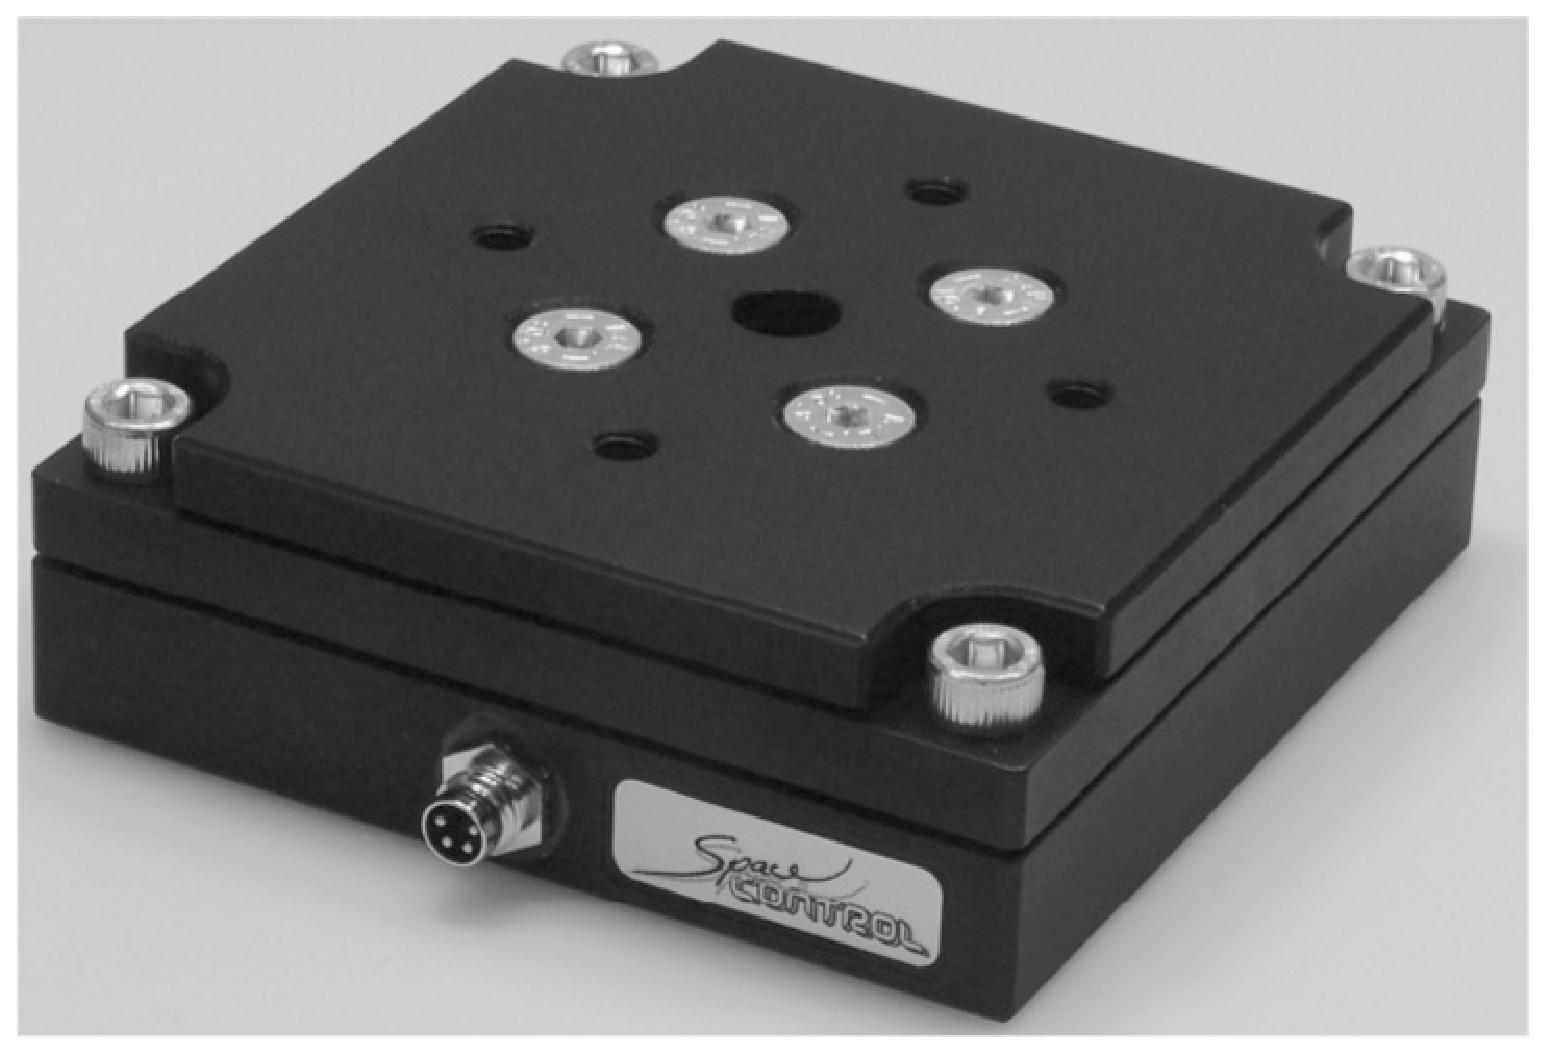
\includegraphics[height=0.16\textheight]{figs/OFTS} &
    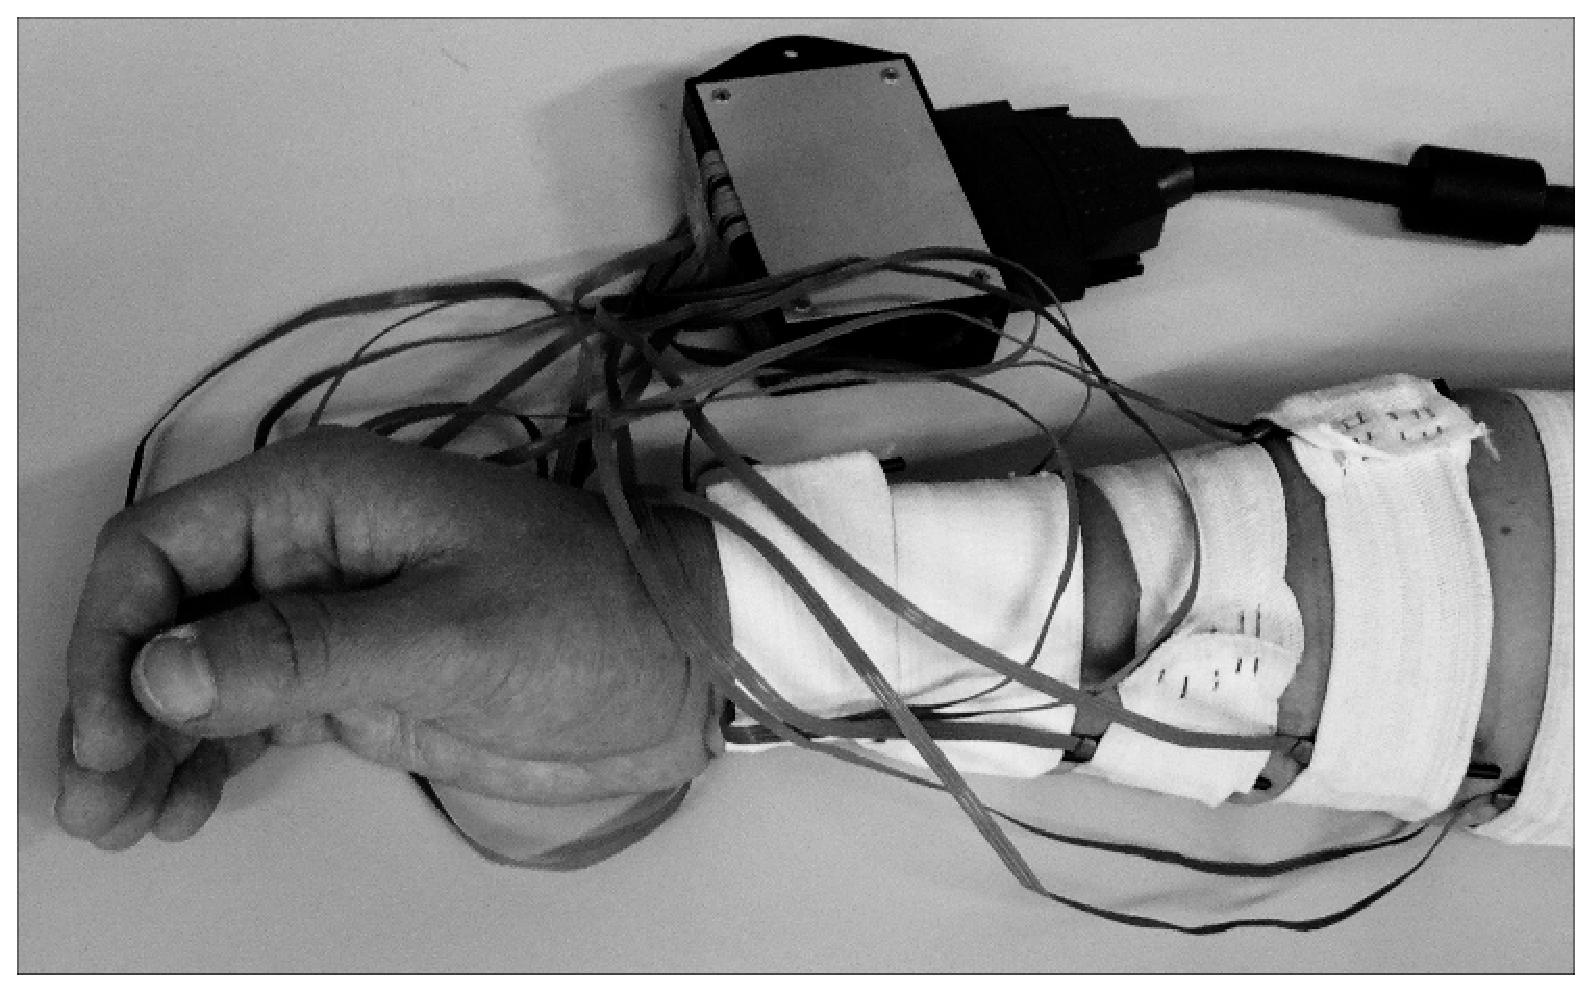
\includegraphics[height=0.16\textheight]{figs/setup} &
    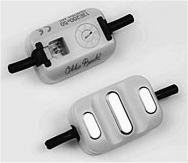
\includegraphics[height=0.16\textheight]{figs/ottobock} \\
    $(a)$ & $(b)$ & $(c)$ \\
  \end{tabular}
  \caption{The experimental setup. $(a)$ The SpaceControl OFTS
    force/torque sensor, large face up. $(b)$
    The arm of the subject with the EMG electrodes fitted and held in
    place by elastic bands. Electrode cables are wired in a box and
    then directed to a National Instruments PCI-6023E analogic/digital
    conversion card (not shown). $(c)$ An Otto Bock 13E200=50
    surface EMG electrode, with the amplification gauge (upper part of
    the Figure) and the three metallic contacts (lower part).}
  \label{fig:setup}
\end{figure*}

\subsubsection{General setup description}

The experiment consisted of freely, repeatedly grasping a SpaceControl
OFTS force/torque sensor \cite{ofts} orthogonally to its large face
(see Figure \ref{fig:setup} $(a)$). Four different ways of pressing
were allowed: opposing the thumb and index, the thumb and middle, the
thumb and ring or the thumb and all other fingers. The speed and force
was intentionally left to the subject's will. Four force sensing
resistors (FSRs) were applied on the subject's hand fingertips (thumb,
index, middle and ring), in order to be able to detect which grasp
type was used at each instant of time. At the same time, $10$ forearm
surface EMG electrodes were applied to the subject's forearm, held in
place by elastic bands, in order to gather information about the
muscle activation (see Figure \ref{fig:setup} $(b)$).

Numerical data from the EMG electrodes, FSRs and OFTS were gathered at
the fastest sampling rate we could obtain, that is, $256$Hz, using a
National Instruments DAQ PCI-6023E analogic/digital conversion card
\cite{nidaq}, mounted on a fast PC equipped with Windows XP.

\subsubsection{EMG signal and electrode placement}
\label{subsubsec:electrodes}

The $10$ EMG electrodes were applied to the subject's right forearm,
held in place by elastic bands. The electrodes were
double-differential Otto Bock 13E200=50 models (\cite{ottobock}, see
Figure \ref{fig:setup} $(c)$), each one gifted with an amplification
gauge ranging from $2000$ to $100000$ times. Initial qualitative
experiments revealed that a safe setting for the amplification gauge
was in the middle of the range, corresponding to about $14000$
times. This is in agreement with the EMG signal amplitude predicted in
the related literature (see, e.g., \cite{deluca}), that is about $100
\mu V$ on average: the voltages our DAQ card read ranged from $0V$ to
about $2.5V$.

Six of the electrodes were placed in pairs along the lower face of the
forearm, whereas four of them were applied in pairs on the upper
face. The initial positioning of the electrodes was chosen in order
for them to lie approximately on top of the muscles which elicit
finger movements; the precise placement was done following the
description in \cite{smagt}, which proved to be optimal for Support
Vector Machine classification of hand postures.

As far as the EMG signal is concerned, it must be remarked that it is
subject to remarkable changes depending on, at least, four orders of
factors:

\begin{enumerate}

  \item \emph{inter-subject variability.} All forearms are different
    from one another in shape, size and power.

  \item \emph{arm posture.} Besides finger movements and grasping, the
    forearm muscles are also involved in the motion of the arm. The
    EMG signal is therefore likely to change if the forearm is moved
    during signal acquisition, for example when switching from
    pronation to supination, or simply while walking around. Even
    raising the shoulder to lift the forearm from the table will
    result in remarkable signal changes.

  \item \emph{electrode displacement.} The intensity and quality of
    the EMG signal depends upon a correct placement of the electrode
    over a muscle. In principle, each electrode should be placed over
    a single muscle, precisely on top of the muscle belly, halfway the
    length of the muscle, and always exactly in the same place.
    Displacing the electrodes will alter the signal, and beside that,
    a precise placement is essentially impossible when dealing with
    surface forearm EMG.

  \item \emph{muscle fatigue.} As the muscles are used more and more,
    continually, fatigue changes the RMS of the EMG signal, calling
    for continual adaptation, at least over a reasonable set of
    different fatigue conditions.

\end{enumerate}

Problems $1$ and $2$ have been for now neglected by concentrating on
one subject only, male, aged $35$ and fully able-bodied, instructed to
keep the arm still and relaxed on a table in a confortable position,
with the palm orthogonal to the plane of the table. See the Discussion
Section for more about these issues.

As far as muscle fatigue and electrode displacement are concerned,
electrodes \emph{cannot} be expected to exactly lie in the very same
position every time the prosthesis is used; moreover, in a preliminary
round of experiments, muscle fatigue was clearly perceived by the
subject during the experiment. In this framework, the only possibility
to overcome these problems is to explicitly take them into account,
gathering enough data to be able to train the machine under different
conditions of electrode displacement and muscular fatigue.

We then organised the experiment as follows: the subject was
instructed to continually grasp the sensor over a period of time of
three to four minutes; then he was allowed to rest for about two
minutes. This was called a \emph{session}. It was expected that muscle
fatigue would appear already during one session. Three sessions were
gathered without taking the elastic bands off the subject's forearm,
in order \emph{not} to have electrode displacement within such a set
of sessions, that we called a \emph{group}. After each group, the
electrodes and bands were removed and the subject was allowed for a
much longer period of rest, ranging from half an hour to one
hour. During resting in-between groups, the subject could get back to
his normal muscular activity.

Five groups were then gathered during one day; and this procedure was
entirely repeated during another day. This procedure would allow us to
examine a relevant amount of data, gathered along a relatively long
period of time and under different conditions of muscle fatigue
(within one session) and electrode displacement (between groups). As
an example, Figure \ref{fig:drift}, pane $(a)$, shows the typical
electrode output during a session (moving average over about $10$
seconds). One can notice strong low-frequency components due to muscle
fatigue.

Spectral analysis of the EMG signal revelaed that all relevant
information is limited to $10$Hz (damping of $-30$dB at that
frequency), therefore sampling at $256$Hz proved to be a large
overshoot. We will employ this fact later on.

\begin{figure}[!ht] \centering
  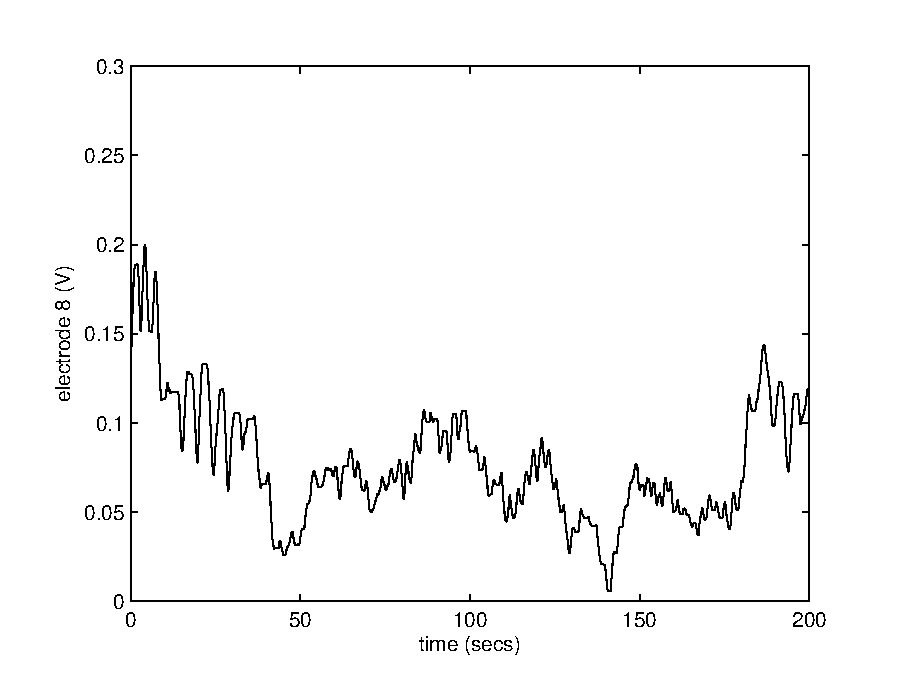
\includegraphics[width=0.45\textwidth]{figs/el8_movingAvg_s1}
  \caption{Typical behaviour of an electrode signal over a
    session (moving average over about $10$ seconds). Drifting can be
    clearly seen in the signal, due to muscle fatigue.}
  \label{fig:drift}
\end{figure}

\subsubsection{Force applied during the grasp}

The OFTS force/torque sensor would output a (negative) integer
numerical value ranging from $0$ to about $-5000$, expressed in
(negative) fiftieths of a Newton. After normalisation, the range of
the applied force would then be between $0N$ and $100N$, with a
resolution of $0.02N$. Linearity of the sensor is guaranteed, and was
anyway manually verified.

\subsubsection{Type of grasp}

The voltage values output by the $4$ FSRs applied onto the subject's
fingertips were monitored in order to understand which kind of grasp
the subject was applying to the sensor. A threshold was experimentally
decided, above which the finger would be defined \emph{in contact}
with the sensor. Using this technique, for each instant in time one of
five possible categories was established: $0$, no action; $1$, grasp
by opposing the thumb and index finger; $2$, opposing thumb and
middle; $3$ thumb and ring; and lastly $4$, grasp by opposing the
thumb and all other fingers.

It must be remarked here that the EMG signal would be altered
immediately at the onset of finger movement, which our setup was
unable to detect. This would result in potential wrong EMG values for
category $0$. Moreover, the FSRs have been experimentally determined
to suffer from a remarkable hysteresis effect, that is, they will
indicate slightly different voltage while pressing and releasing; this
is due to small rubber ends glued on top of the sensor surfaces, which
aid grasping by raising the static friction coefficient. Hysteresis is
also supposed to somehow degrade the quality of the learning. Because
of these factors we would never expected a close-to-$100\%$
classification accuracy, nor a perfect reconstruction of the applied
force. A better setup is currently being studied, which would avoid
these effects. Again, see the Discussion for more about this issue.


\subsection{Learning Methods}
\label{subsec:analysis}
The gathered data was analysed both for classification and
regression. \emph{Classification} is the process by which one wants to
assign a label to each sample in the input space, whereas in
\emph{regression} the target is a real-valued function of the values
of the input samples. Throughout this Section, we will assume that a
set of $l$ points in the input space is available, for which the
target (label or force value) is known; this set will be denoted by
$\{\xx_i,y_i\}_{i=1}^l$ and called \emph{training set}. As well, for
each experiment, a separate set of points, for which the targets are
not known, is assumed to be available, and this will be called the
\emph{testing set}. In general, the performance of a machine is tested
by training it on a training set and then testing it on a testing set,
possibly employing standard measures of the generalisation error, such
as cross-validation.

Taking into account the considerations of the previous Section, we set
the input space to be $\RR^{10}$, that is, one coordinate for each EMG
electrode; therefore, $\xx_i \in \RR^{10}, i=1,\ldots,l$. In the case
of classification, each category representing a grasping type would be
represented as an integer value, that is, $y_i \in \{0,\ldots,4\}
\subset \NN, i=1,\ldots,l$. In the case of regression, the force value
would be directly encoded as a real number, that is, $y_i \in \RR,
i=1,\ldots,l$. Before any analysis, all samples were normalised, as is
customary, by subtracting the mean values and dividing by the standard
deviation, for each input space dimension. No filtering whatsoever was
applied to the input signals, in order to have a more realistic,
delay-free result.

\subsubsection{Neural Networks}

Artificial Neural Networks (NNs or ANNs for short; see, e.g.,
\cite{bishop} for a comprehensive introduction) are probably the most
popular machine learning algorithm nowadays available for both
classification and regression. An ANN is a directed graph in which,
for every node, the weighted sum of the input values is evaluated;
this sum is then used as the argument of an \emph{activation function}
to determine the output of the node. The nodes fed the input values to
the network are called \emph{input layer}, and the nodes whose output
is taken as the output of the network are called \emph{output
layer}. Besides this, in general, an ANN can further have an arbitrary
number of nodes organised in \emph{hidden layers}, gifted with an
arbitrary edge topology.

An ANN is initialised with random weights; then, for every sample in
the training set, the network output is evaluated and its error with
respect to the target is considered. In order to reduce the error
then, a minimisation algorithm is then employed to change the weights
of the network, until the desired precision is reached. If the
generalisation error has been kept small, the network will then be
able to \emph{predict} the targets of the testing samples with a
reasonable accuracy.

For our experiment we strived to keep the ANN as simple as possible.
We then chose a basic feed-forward NN with $10$ units for the input
layer; one hidden layer with $10$ units with sigmoidal arcotangent
activation function; $5$ units in the output layer for classification,
each unit representing one category, and one unit in the output layer
for regression, the unit representing the target force value. The
network was trained via the \textbf{BOH} algorithm and learning
function \textbf{BOHBOH}; the mean-square error (MSE) was used as a
measure of performance. The training phase was stopped arbitrarily
after $30$ epochs. For each experiment, we repeated the training phase
$10$ times, in order to overcome the well-known problem of local
minima, and then gathered the best model found. No measure of
generalisation error was taken into account.

The network was implemented in Matlab, Windows version $7.1.0.246$
(R14) Service Pack 3, running on a bi-processor $1.8$GHz machine with
1GB on-board memory; we used the Matlab Neural Network Toolbox,
version $5.0.1$ (R2006b).

\subsubsection{Support Vector Machines}

Support Vector Machines (SVMs; see, e.g.,
\cite{BGV92,Burges98,Cristianini00}) are a machine learning method
able to determine the best candidate function for a classification or
regression problem, drawn from a functional space induced by the
choice of a binary function between points in the sample space,
$K(\xx_1,\xx_2)$, with $\xx_1, \xx_2 \in \RR^{10}$ in this case. $K$
is called \emph{kernel}. In the most general setting, the function
found is

\begin{equation} \label{eqn:sol}
  f(\xx) = \sum_{i=1}^l \alpha_i y_i K(\xx,\xx_i) + b
\end{equation}

\noindent where $b \in \RR$, whereas the $\alpha_i \in \RR$s are
Lagrangian coefficients obtained by solving a minimisation problem
whose cost functional is guaranteed to be convex. Because of this,
SVMs do not suffer from the problem of local minima; but their
training time is cubic in the number of samples in the training set,
as opposed to ANNs, for which it is \textbf{BOHBOH}.

In order to overcome this problem, which would have made our
experiment unfeasible, we have decided to use a \emph{uniformisation}
strategy on the training sets, before training the machines. The idea
is that, in a real-life set-up such as ours, there can be many input
samples located in the very same region of the input space, with very
similar target values. One obvious case is that of label $0$,
indicating no ongoing grasping: it is intuitively expected that a
large number of samples will be taken in that region of the input
space, since the subject will be in the $0$ condition for a longer
time than all other labels.

Since all functions involved in the experiment are due to human
motion, we can assume that they are continuous and, probably,
derivable up to any arbitrary order. Therefore it makes no sense for
an approach such as SVMs to sample the input space in a non-uniform
way such as that described above. The uniformisation procedure
consists of removing, from a training set, those samples which are too
close to each other, according to a suitable notion of inter-sample
distance.

In order to take into account the different variances of the EMG
electrode values, we have decided to adopt Mahalanobis's distance as
the inter-sample distance \cite{...}. Let $\xx_1, \xx_2 \in \RR^{10}$;
then the Mahalanobis distance between $\xx_1$ and $\xx_2$ is defined
as follows:

$$ MD(\xx_1,\xx_2) = \sqrt{(\xx_1-\xx_2)^T \Sigma^{-1} (\xx_1-\xx_2)} $$

\noindent where $\Sigma$ is the $10$x$10$ covariance matrix, evaluated
on the training set. $MD(\xx_1,\xx_2)$ is a distance in which each
summand is weighted inversely with respect to the variance of the
samples along that dimension of the input space: it is therefore a
measure of distance independent of the variance of the single
electrodes. Notice that if $\Sigma$ is replaced by the identity
matrix, $MD(\xx_1,\xx_2)$ is reduced to the usual notion of Euclidean
distance.

Since checking the inter-sample distance obviously takes a quadratic
time with respect to the number of samples, which was unfeasible, we
adopted an approximated method which was able to remove most, but not
all, samples with an insufficient Mahalanobis distance from any other
sample. After a few initial experiments we set the threshold distance
at $1$. All our experiments with SVMs were then performed on
uniformised training sets, using $5$-fold cross-validation and grid
search to find the optimal values of the standard Gaussian kernel
hyperparameters, $C$ and $\sigma$.

On the other hand, notice that no \emph{testing} set was uniformised,
since it would probably be unfeasible to apply the same procedure in
an on-line setting. Notice, further, that applying uniformisation
resulted in training sets which were considerably smaller than the
original ones, up to about $100$ times smaller.

Lastly, we employed a well-known freely available SVM package,
\emph{libsvm} v2.83 \cite{...}, in the Matlab wrapped flavour.

\subsubsection{Locally Weighted Projection Regression}

\textbf{LWPR - prendi qualcosa dalla rete. spiega gs e cv.}



\section{Experimental Evaluation}
\label{sec:exp}

In this Section we describe the experimental analysis. In particular,
we first describe some preliminary results obtained in batch fashion,
which have led to the development of Online Uniformisation (OU). We
then show a detailed comparative analysis of the three approaches
selected, first on the classification problem, and then on the
regression problem, in which OU is used.

\subsection{Batch Experiments}
\label{subsec:strategy}
\subsubsection{Batch Uniformisation}

First of all we chose one of the selected approaches (NNs, SVMs or
LWPR) and one problem (classification or regression) for initial
experimentation. We decided to use SVMs for classification. We then
decided to test whether data obtained during one session could be used
to build a model able to generalise over other sessions during the
same day.

Here an obvious problem arises: the total time of the experiment
during which data were gathered was about $100$ minutes; at $256$Hz,
that means about $1.6$ millions samples, an unfeasibly large training
set for any of the examined methods, not to mention SVM
classification. Even restricting a training set to a single session,
this would result in about $53000$ samples, which not only is still
too large, but probably contains redundant and irrelevant
information. Moreover, in a real setting, this number is doomed to
grow continually and cannot therefore be used as it is for periodical
re-training. We then decided to investigate a smart sampling strategy
in order both to overcome this problem, but also to gain insight into
the EMG signal in general. This led us to develop the batch version of
the uniformisation procedure.

The simple idea behind batch uniformisation is that, in a real-life
set-up such as ours, there can be many input samples located in the
very same region of the input space, with very similar target
values. One obvious case is that of label $0$, indicating no ongoing
grasping: it is intuitively expected that a large number of samples
will be taken in that region of the input space, since the subject
will be in the $0$ condition for a longer time than all other
labels. Since all functions involved in the experiment are due to
human motion, we can assume that they are continuous and, probably,
derivable up to any arbitrary order. Therefore it makes no sense to
consider samples obtained in a non-uniform way such as that described
above. The batch uniformisation procedure consists of removing, from a
training set, those samples which are too close to each other,
according to a suitable notion of inter-sample distance.

In order to take into account the different variances of the EMG
electrode values, and since in batch data analysis all data are
available beforehand and therefore all possible statistics can be
gathered a-priori, we have decided to adopt Mahalanobis's distance as
the inter-sample distance. Let $\xx_1, \xx_2 \in \RR^{10}$; then the
Mahalanobis distance between $\xx_1$ and $\xx_2$ is defined as
follows:

$$ MD(\xx_1,\xx_2) = \sqrt{(\xx_1-\xx_2)^T \Sigma^{-1} (\xx_1-\xx_2)} $$

\noindent where $\Sigma$ is the $10$x$10$ covariance matrix, evaluated
on the training set. $MD(\xx_1,\xx_2)$ is a distance in which each
summand is weighted inversely with respect to the variance of the
samples along that dimension of the input space: it is therefore a
measure of distance independent of the variance of the single
electrodes. Notice that if $\Sigma$ is replaced by the identity
matrix, $MD(\xx_1,\xx_2)$ is reduced to the usual notion of Euclidean
distance.

Since checking the inter-sample distance obviously takes a quadratic
time with respect to the number of samples, which was unfeasible, we
adopted an approximated method which was able to remove most, but not
all, samples with an insufficient Mahalanobis distance from any other
sample. After a few initial experiments, the threshold distance was
set at $1$. Notice that no \emph{testing} set was uniformised, since
it would probably be unfeasible to apply the same procedure in an
on-line setting. Notice, further, that applying uniformisation
resulted in training sets which were considerably smaller than the
original ones, up to about $100$ times smaller.

The first question is: do uniformised training sets lack any relevant
information? We trained a SVM over each single session, both for the
first and second day, and both with full and uniformised training
sets. The session were numbered chronologically during the day,
sessions $1,2,3$ forming group $1$, sessions $4,5,6$ forming group
$2$, and so on. With a slight abuse of language, we will call the
model obtained by training a machine on session $i$, \emph{model
$i$}. Moreover, in the remainder of this Subsection, if the training
set of a model was uniformised, we will call the model \emph{uniform}.

We then tested each model on all sessions of the same day, obtaining
therefore an \emph{accuracy matrix} $A$ in which $A_{ij}$ would be a
percentage denoting the correctly guessed labels when testing model
$i$ (standard or uniform) on session $j$. Notice once again that, in
the case of uniform models, the test is carried out on the \emph{full}
session. This is what we would call a \emph{cross-session analysis}.
The result is visible in Figure \ref{fig:cross_initial}.

\begin{figure*}[!ht] \centering
  \begin{tabular}{cc}
    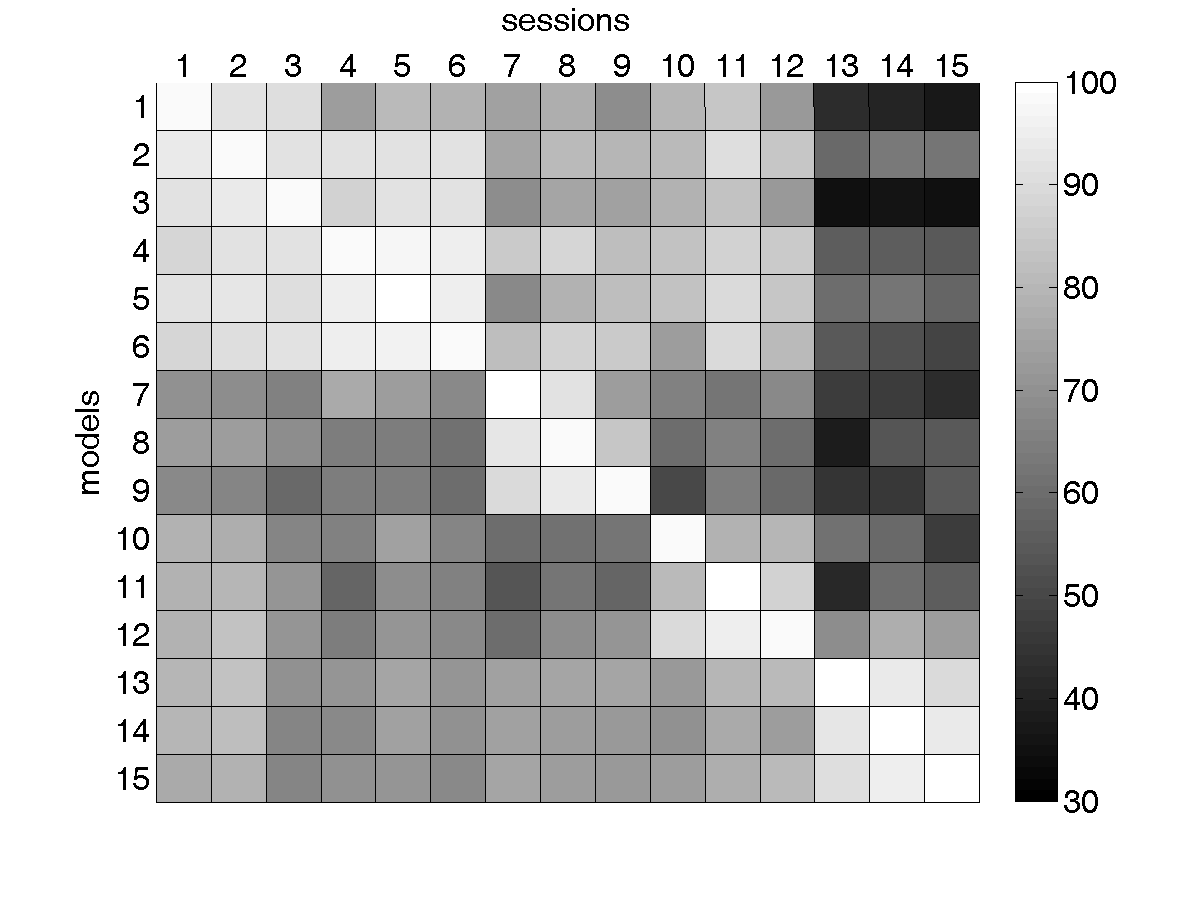
\includegraphics[width=0.45\textwidth]{figs/fig_resCross1_full} & 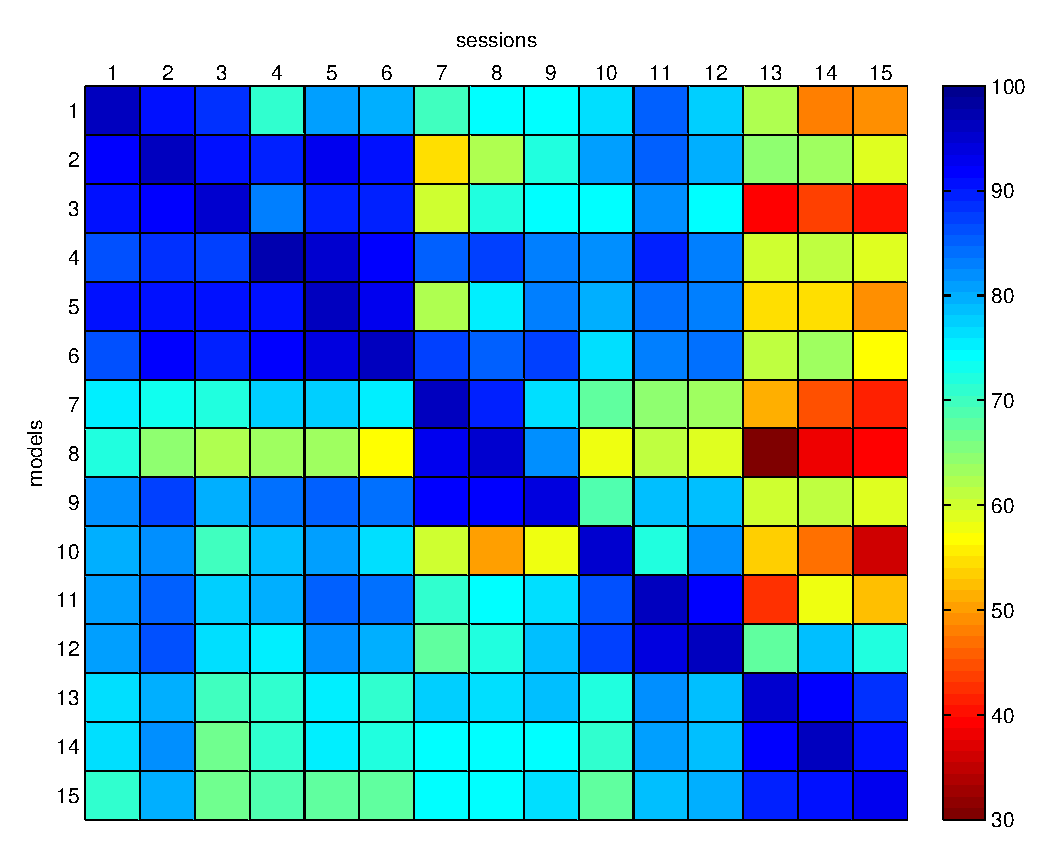
\includegraphics[width=0.45\textwidth]{figs/fig_resCross1} \\
    diagonal: $98.73\% \pm 0.39\%$  & diagonal: $95.52\% \pm 1.21\%$ \\
        rest: $73.23\% \pm 14.29\%$ & rest: $74.53\% \pm 13.70\%$ \\
    $(a)$ & $(b)$ \\
    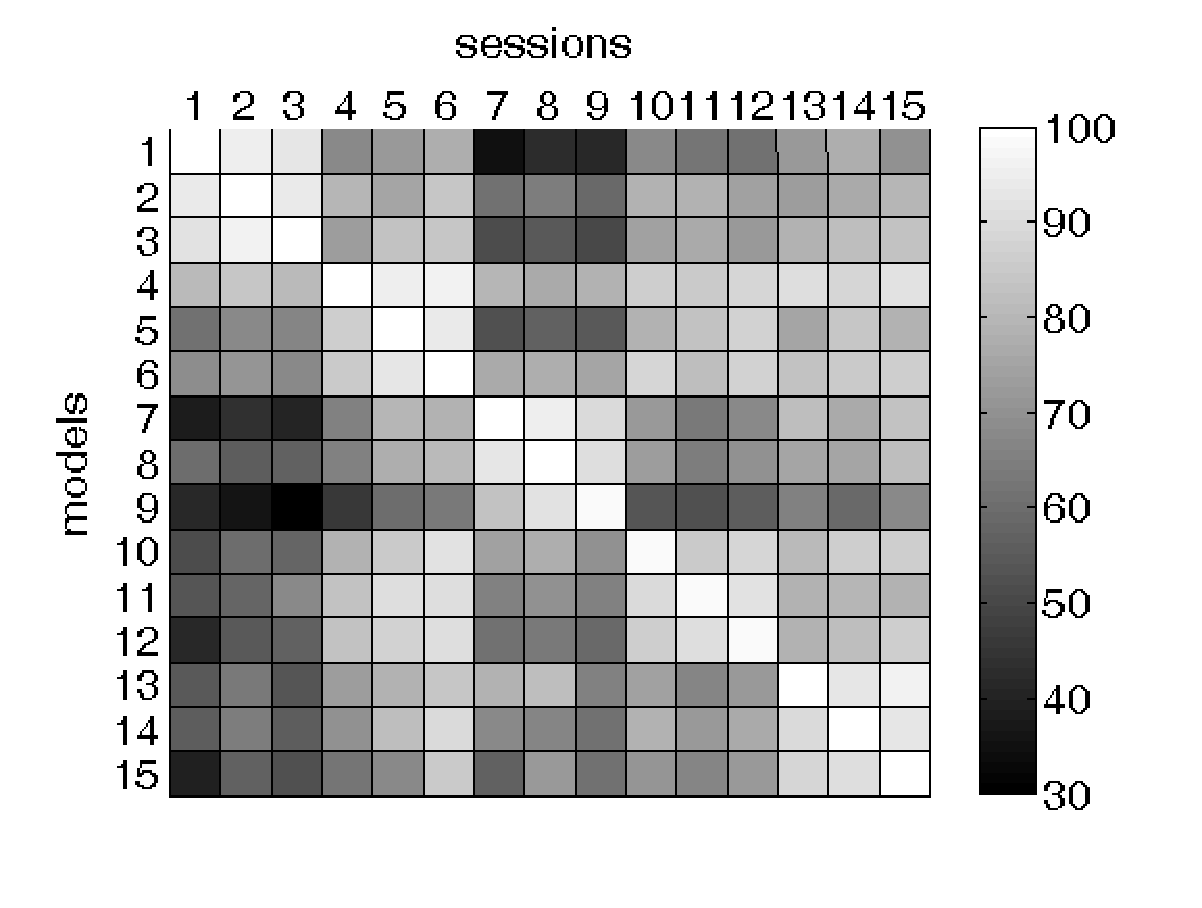
\includegraphics[width=0.45\textwidth]{figs/fig_resCross2_full} & 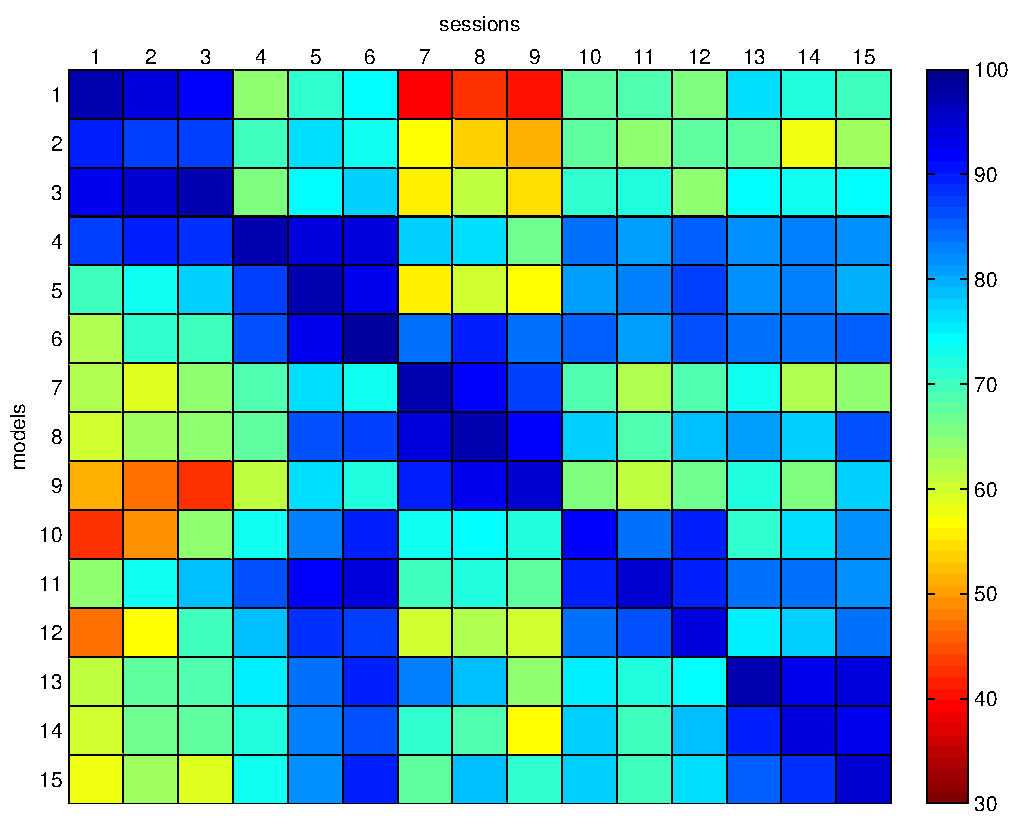
\includegraphics[width=0.45\textwidth]{figs/fig_resCross2} \\
    diagonal: $99.05\% \pm 0.37\%$ & diagonal: $95.37\% \pm 2.85\%$ \\
        rest: $73.23\% \pm 14.47\%$ & rest: $74.38\% \pm 12.27\%$ \\
    $(c)$ & $(d)$ \\
  \end{tabular}
  \caption{Cross-session analysis and evaluation of the uniformisation
    procedure. $(a)$ and $(b)$, accuracy matrices for day $1$: $(a)$
    full models, $(b)$ uniform models. $(c)$ and $(d)$, same for day $2$.}
  \label{fig:cross_initial}
\end{figure*}

Consider first panes $(a)$ and $(b)$ of the Figure, pane $(a)$ being
the accuracy matrix for full models, day $1$, and pane $(b)$ being the
accuracy matrix for the same day, but using uniform models. It is
apparent from the colours that the full models attain a better
accuracy when tested on their own training data, that is, on the
diagonal of the matrix, than the uniform models. In fact, the mean and
standard deviation of the diagonal accuracies are $98.73\% \pm 0.39\%$
for the full models and $95.52\% \pm 1.21\%$ for the uniform
models. This is intuitively sensible since, in the case of full
models, we are testing on the same data used for training, whereas in
the case of uniform models, the training data are a strict subset of
the testing data, and a quite smaller subset indeed. But as well, if
we consider the remaining elements of the matrices, it is clear that
the uniform models attain a better accuracy \emph{overall}, if
compared to the full models. In fact, the accuracies are $73.23\% \pm
14.29\%$ for the full models, and $74.53\% \pm 13.70\%$ for the
uniform ones. The same analysis for day $2$ yields analogous results
(consider the above Figure, panes $(c)$ and $(d)$).

From this we conclude that the uniformisation procedure is effective
in reducing the training set size, \emph{without actually degrading
the performance}. This is apparent from the fact that uniform models
are more accurate on testing sets which are disjoint from the training
sets. In fact, one should always ensure that this is the case, aiming
for a better generalisation error. We can say that uniform models
generalise better, at least in this case.

\subsubsection{Classification accuracy}

Consider Figure \ref{fig:cross_initial} again, right hand side panes
($(b)$ and $(d)$) and the numbers below. The accuracy attained on
non-diagonal elements is about $74\%$, which is rather bad. One cannot
expect to correctly drive a prosthesis if one sample in four is
misclassified. At the same time, however, a strong ``good group
accuracy'' is obviously present: in each matrix, good accuracy values
are obtained on 3x3 submatrices located on the diagonals,
corresponding to cross-session accuracy for sessions \emph{belonging
to the same group}, that is, where the elastic bands were not removed
and no electrode displacement was present.

More in detail, as far as the first day is concerned (same Figure,
pane $(b)$), one can see that the first six models (trained on the
first two groups) obtain a quite good accuracy on the first six
sessions (first two groups) whereas their accuracy rapidly degrades as
more sessions are tested for. This is probably due to the first two
groups having been gathered in similar conditions, very similar
electrode positions and/or similar movements performed by the
subject. On the other hand, sessions in the last group (columns $13$,
$14$ and $15$ of the matrix) are particularly hard, except when tested
by models obtained from the last group itself --- here the effect is
probably motivated by the opposite reason: during those sessions, the
subject must have explored more relevant parts of the input
space. This is corroborated by the fact that models $13,14,15$ perform
rather well on \emph{all} sessions, if compared to other models (check
rows $13,14,15$ of the matrix). In other words, sessions $13,14,15$
contain more relevant information than the others.

Analogous considerations can be made by inspecting the accuracy matrix
of the second day, pane $(d)$ of the Figure.

From this we can confirm that \emph{electrode displacement plays a
determinant role} in the classification accuracy. Notice that muscle
fatigue seems not to enter the picture, but this is reasonable since
its effetcs are visible already within one single session (see Figure
\ref{fig:drift} again) and the machine correctly takes it into account
during the training phase. Notice once again that the uniformisation
procedure does not hinder the generalisation power of the system.

It is intuitively expected that the poor cross-session generalisation
performance is due to the problem of electrode displacement. This is
experimentally confirmed by the strong degradation in classification
accuracy among different groups. In other words, the SVM does not
generalise well when trained on a session belonging to group and
tested on a session belonging to a different group. Electrode
displacement present between groups (but not within a group) causes
the samples in a group to be ``shifted'' in the input space, so that
testing on a different group results in poor generalisation
performance. To substantiate this claim, we have verified that the
cross-session accuracy is highly correlated to the
\emph{average minimum inter-sample distance} between sessions. More in
detail, let $S_i$ denote the training set for session $i$; we have
built a distance cross-session matrix $D$ in which

$$ D_{ij} = \frac{1}{|S_j|} \sum_{s_j \in S_j}{\min_{s_i \in S_i}{ ||s_j-s_i||^2 } } $$

Essentially, $D_{ij}$ denotes how far away in the input space the
samples in $S_j$ are from the samples in $S_i$. Note that $D$ is in
general not symmetric, since we consider the \emph{average} of the
\emph{minimum} distance of each sample in $S_j$ from those in $S_i$.

The cross-correlation coefficient evaluated between the values of $D$
and the accuracy values of the cross-session accuracy matrix is
$-0.61$ \emph{both} for the first and the second day, indicating a
strong negative correlation. Further experiments have revealed that
this happens for Neural Networks too (cross-correlation $-0.40$ for
day $1$ and $-0.51$ for day $2$); and also, that $D$ is strongly
\emph{positively} correlated to the MSE in regression, for all the
studied approaches: $0.62/0.78$ (day $1$/day $2$) for SVMs,
$0.64/0.72$ for NNs and $0.77/0.81$ for LWPR.

In other words, the larger the distance of $S_i$ and $S_j$, the worse
the performance of model $i$ tested on session $j$, both in
classification and in regression. This tells us that $(a)$ samples of
the same group are closer to each other than sample from different
groups, therefore electrode displacement causes displacement in the
input space too; and $(b)$ that this causes bad inter-group
performance. ``Samples far away from the training set will be
predicted badly.''

%% In order to further sustain this claim we have checked, for each day,
%% that models obtained by adjoining $4$ of the $5$ groups would perform
%% well on the group excluded when training; this would indeed indicate
%% that more data is needed to train the machine, and that the required
%% data must somehow be found in some of (but not necessarily all) the
%% gathered groups. We will call these models \emph{multi-group
%% models}. The results are visible in Figure \ref{fig:bigmodels}.

%% \begin{figure*}[!ht] \centering
%%   \begin{tabular}{cc}
%%     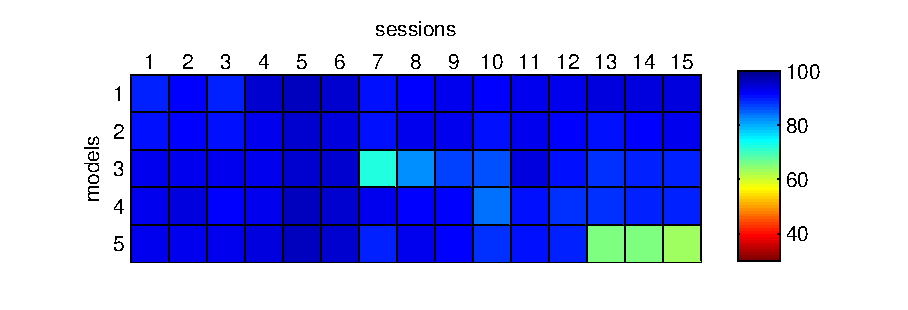
\includegraphics[width=0.45\textwidth]{figs/fig_resCross_day1_big} & 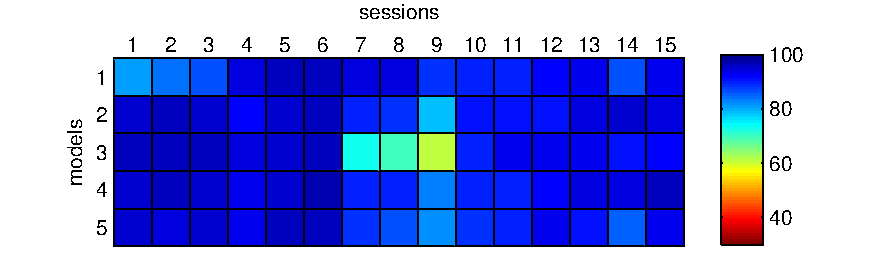
\includegraphics[width=0.45\textwidth]{figs/fig_resCross_day2_big} \\
%%     $(a)$ & $(b)$ \\
%%   \end{tabular}
%%   \caption{Cross-session analysis of multi-group models, obtained by adjoining $4$
%%     of the $5$ groups of each day. Each row denotes the model trained
%%     excluding group $1,\ldots,5$ from the model itself. $(a)$ day $1$, $(b)$ day $2$.}
%%   \label{fig:bigmodels}
%% \end{figure*}

%% Consider the rows of the matrices in the Figure: as one can see, the
%% accuracy is uniformly very high, even when the models are tested on
%% unseen testing data; for instance, model $1$ of day $1$ has an
%% accuracy of $92.82\% \pm 1.96\%$, and model $4$ of day $2$ has an
%% accuracy of $92.64\% \pm 3.73\%$. Moreover, notice that, e.g., model
%% $5$ of day $1$ performs badly on group $5$ of day $1$, as one can
%% expect, since model $5$ has not been trained on that very group, which
%% was already determined to be very hard (compare Figure
%% \ref{fig:cross_initial}, pane $(b)$, last three columns).

%%  Model $1$ of day $1$, for
%% instance, performs uniformly very well. From this we first conclude
%% that the uniformisation procedure is not eliminating any useful
%% information from the training sets; and, secondly, that if the right
%% training data can be found, there are good chances of building a good
%% model.

The dual consideration is that if we train upon the ``right'' data,
the accuracy should become acceptable. So we have considered how to
collect \emph{only} relevant information from the gathered data, that
is, how to sensibly reduce the training set. To do this, we have
collected the two best models for each day and joined them
together. For instance, consider Figure \ref{fig:cross_initial} again,
pane $(b)$. It is apparent that model $4$ performs well on sessions
$1$ to $12$, whereas model $13$ does well on sessions $13$ to $15$. We
then decided to use these two models to form a ``best'' training set
which would give good results on the whole day $1$. Analogous
considerations led us to use also models $4$ and $8$ of day $2$. The
obtained model will be called \emph{best} model.

This procedure was repeated for each problem tackled (classification,
regression) and approach tested (SVM, NN and LWPR). Figure
\ref{fig:best_class} shows the classification accuracy of the best
models for classification on all $15$ sessions of day $1$ and $2$, for
SVMs and NNs. The analysis detailed in the previous Subsection has
been repeated for the Neural Network. In that case, models $8$ and
$15$ of day $1$, and models $3$ and $10$ of day $2$ have been used to
build the best model.

\begin{figure*}[!ht] \centering
  \begin{tabular}{cc}
    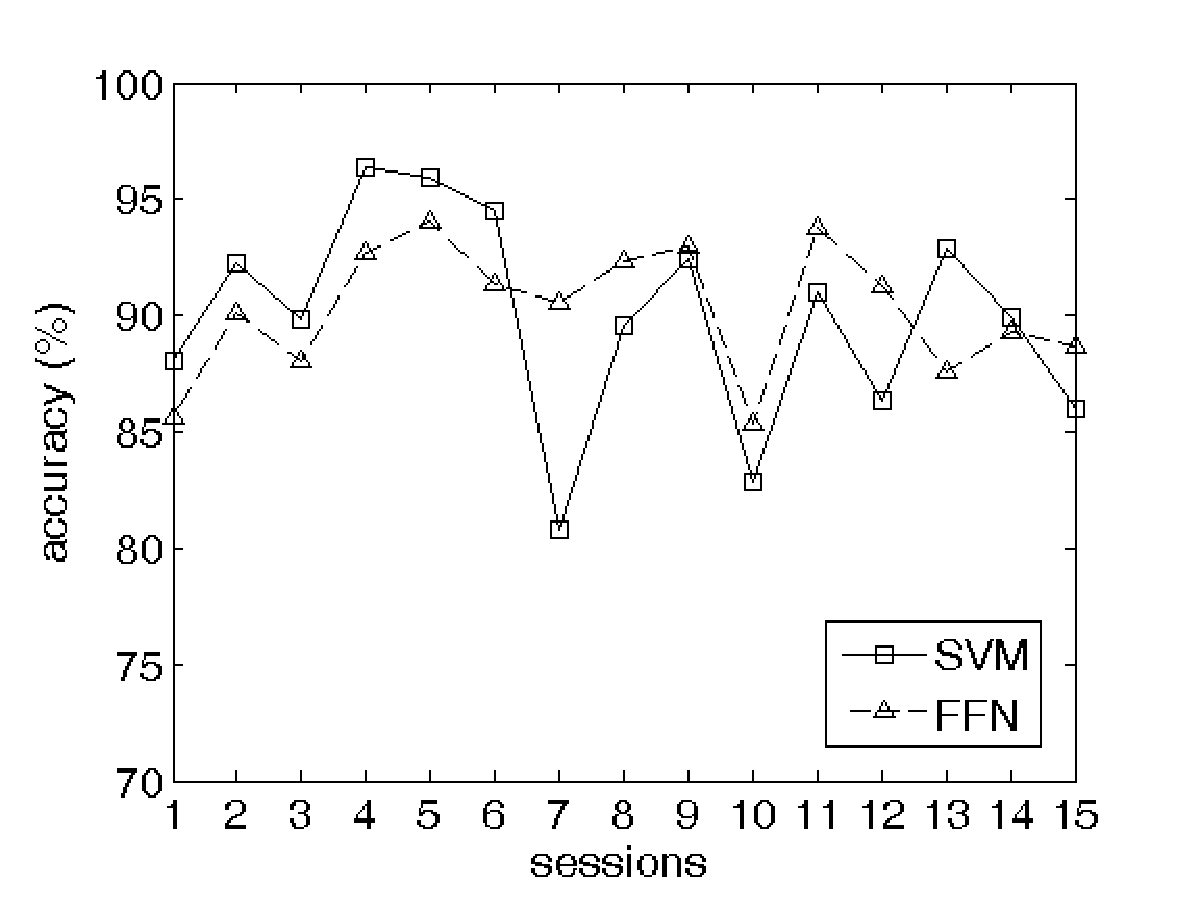
\includegraphics[width=0.45\textwidth]{figs/fig_class_resCrossBestOnDay1} & 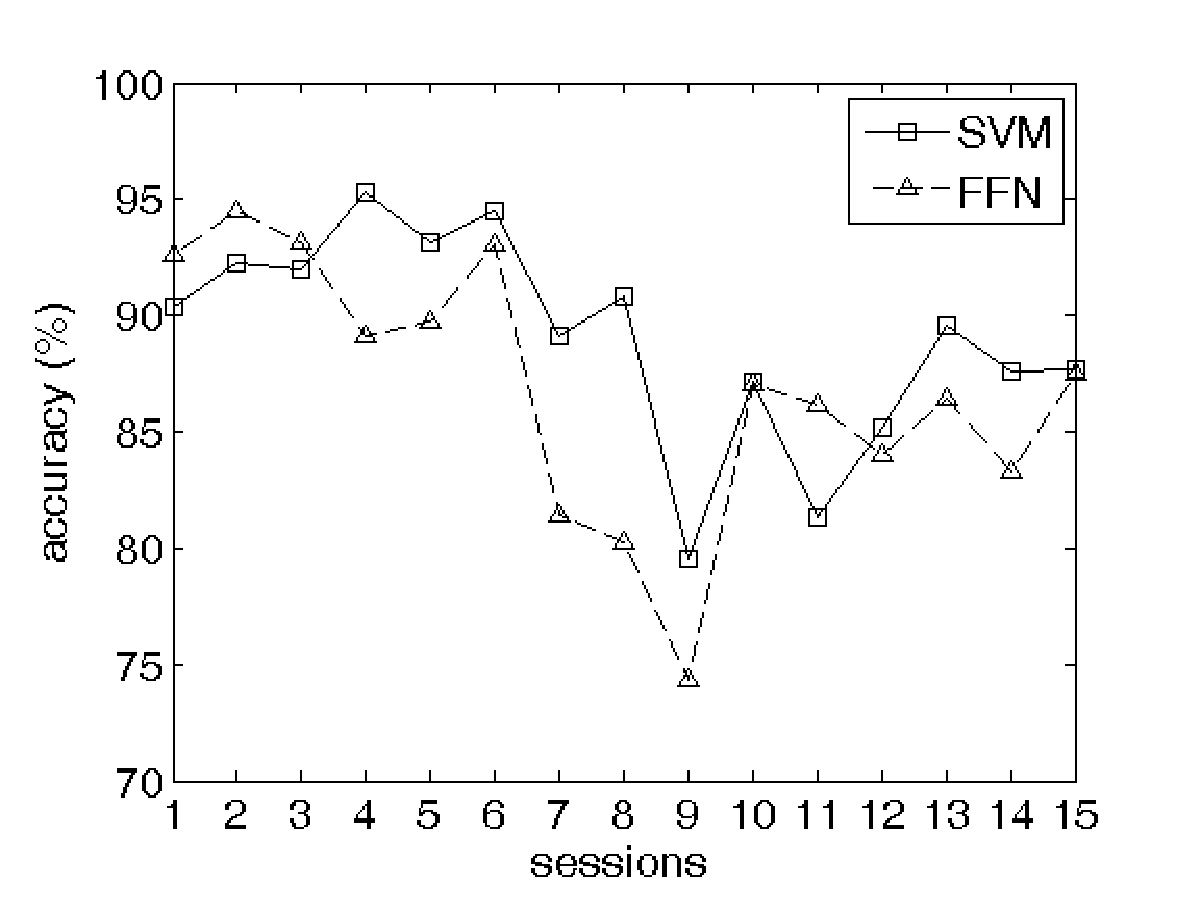
\includegraphics[width=0.45\textwidth]{figs/fig_class_resCrossBestOnDay2} \\
    SVM: $89.90\% \pm 4.51\%$ & SVM: $89.04\% \pm 4.50\%$ \\
    NN: $90.25\% \pm 2.77\%$ & NN: $86.84\% \pm 5.57\%$ \\
    $(a)$ & $(b)$ \\
  \end{tabular}
  \caption{Classification accuracy of best models, day $1$ (pane
  $(a)$) and day $2$ (pane $(b)$).}
  \label{fig:best_class}
\end{figure*}

As one can see, there is no clear winner between SVMs and NNs. NNs
perform slightly better on day $1$ (lower mean, lower standard
deviation) but SVMs are analogously better on day $2$. All in all,
classification accuracy is good, at an overall rate of about
$90\%$. In this case, the training data amounts to four sessions
(uniformised in the case of SVMs and full in the case of NNs), which
is about $12$-$15$ minutes of user activity. But notice, that samples
gathered during both days were necessary to have an idea of which
sessions to use.

Lastly, the most interesting part was how to predict the amount of
force applied by the subject by looking at the EMG signal. To do this,
we have repeated once again the analysis done in Subsection
\ref{subsec:strategy} for the three approaches selected, and found out
that the four sessions involved in the best models were: $6,12,3,12$
for SVMs, $4,11,3,12$ for NNs and $6,13,3,4$ for LWPR.

\subsubsection{Regression}

For regression, we have considered three indicators of performance:
the Mean Squared Error (MSE) in its standard definition; the
Normalised Root MSE (NRMSE), ratio of the square root of the MSE and
the range of the target values, expressed as a percentage; and the
Squared Correlation Coefficient (SCC) between the predicted target and
the real target.

\begin{figure*}[!ht] \centering
  \begin{tabular}{cc}
    \includegraphics[width=0.45\textwidth]{figs/fig_err_regr_resCrossBestOnDay1} &
    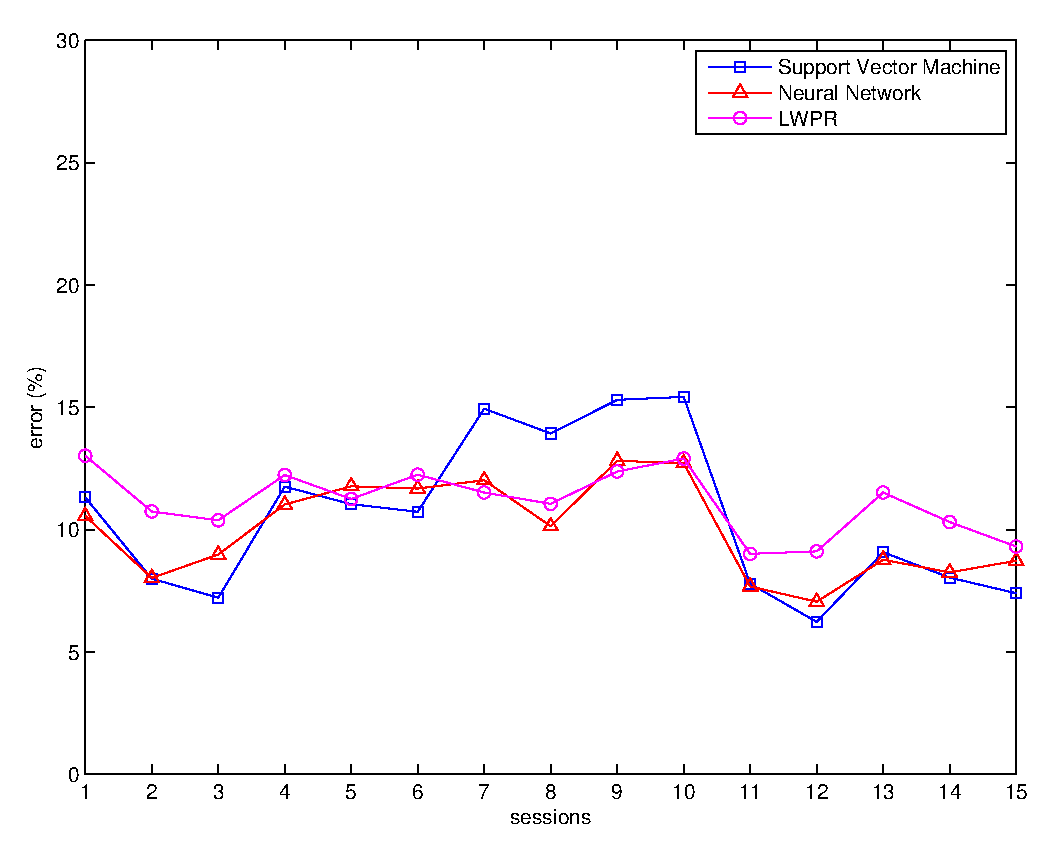
\includegraphics[width=0.45\textwidth]{figs/fig_err_regr_resCrossBestOnDay2} \\
     SVM: $11.84\% \pm 2.64\%$ &  SVM: $10.54\% \pm 3.18\%$ \\
      NN: $10.54\% \pm 1.41\%$ &   NN: $10.01\% \pm 1.93\%$ \\
    LWPR: $11.98\% \pm 1.31\%$ & LWPR: $11.13\% \pm 1.32\%$ \\
    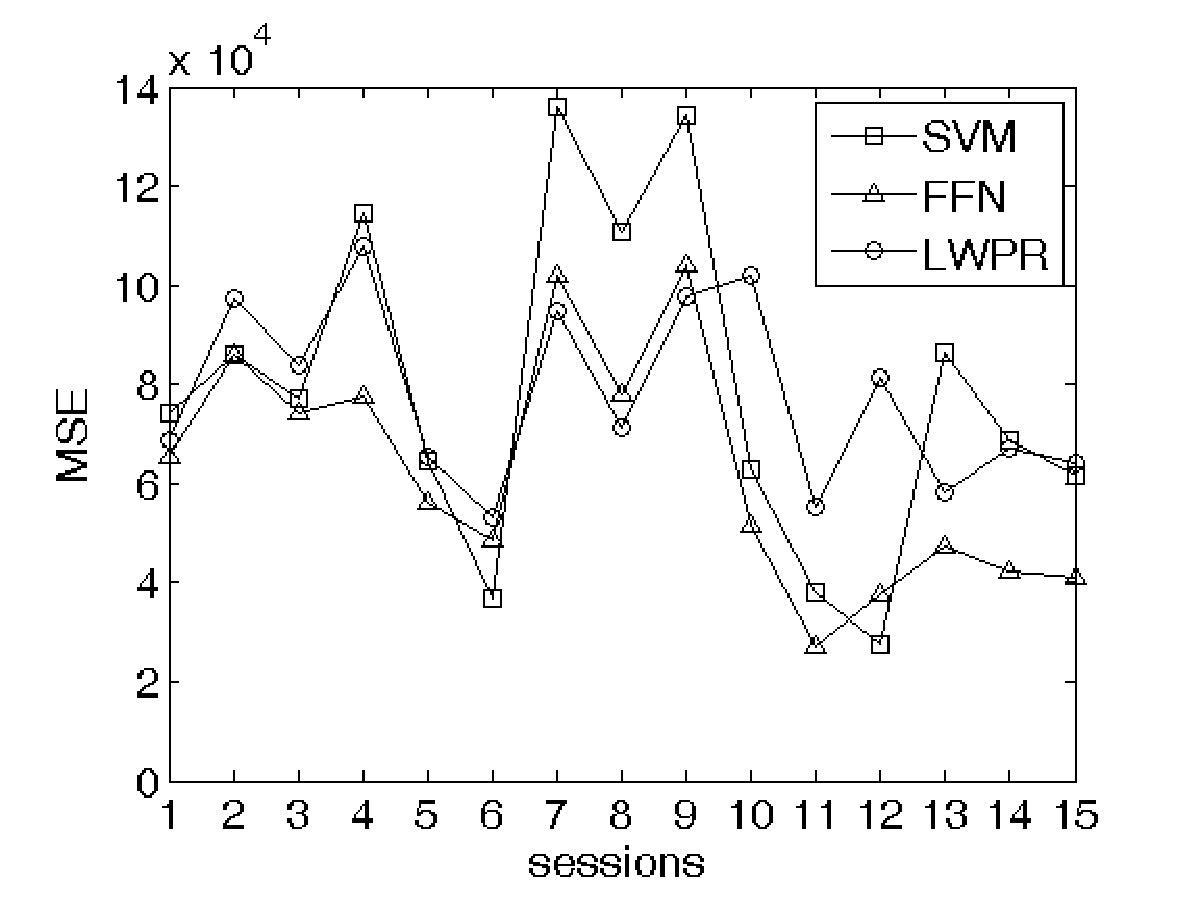
\includegraphics[width=0.45\textwidth]{figs/fig_MSE_regr_resCrossBestOnDay1} &
    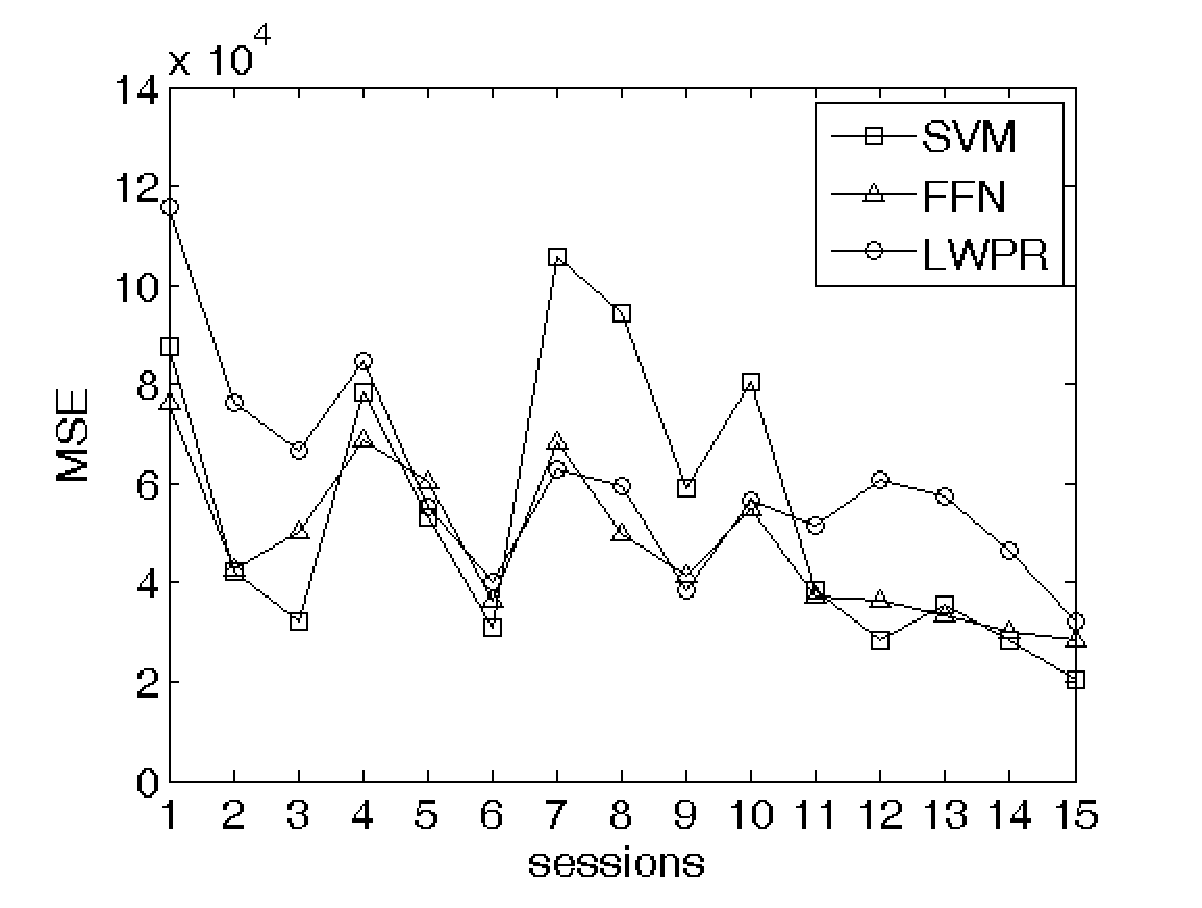
\includegraphics[width=0.45\textwidth]{figs/fig_MSE_regr_resCrossBestOnDay2} \\
     SVM: $7.86 \pm 3.35$ &  SVM: $5.44 \pm 2.79$ \\
      NN: $6.27 \pm 2.36$ &   NN: $4.76 \pm 1.52$ \\
    LWPR: $7.79 \pm 1.83$ & LWPR: $6.03 \pm 2.07$ \\
    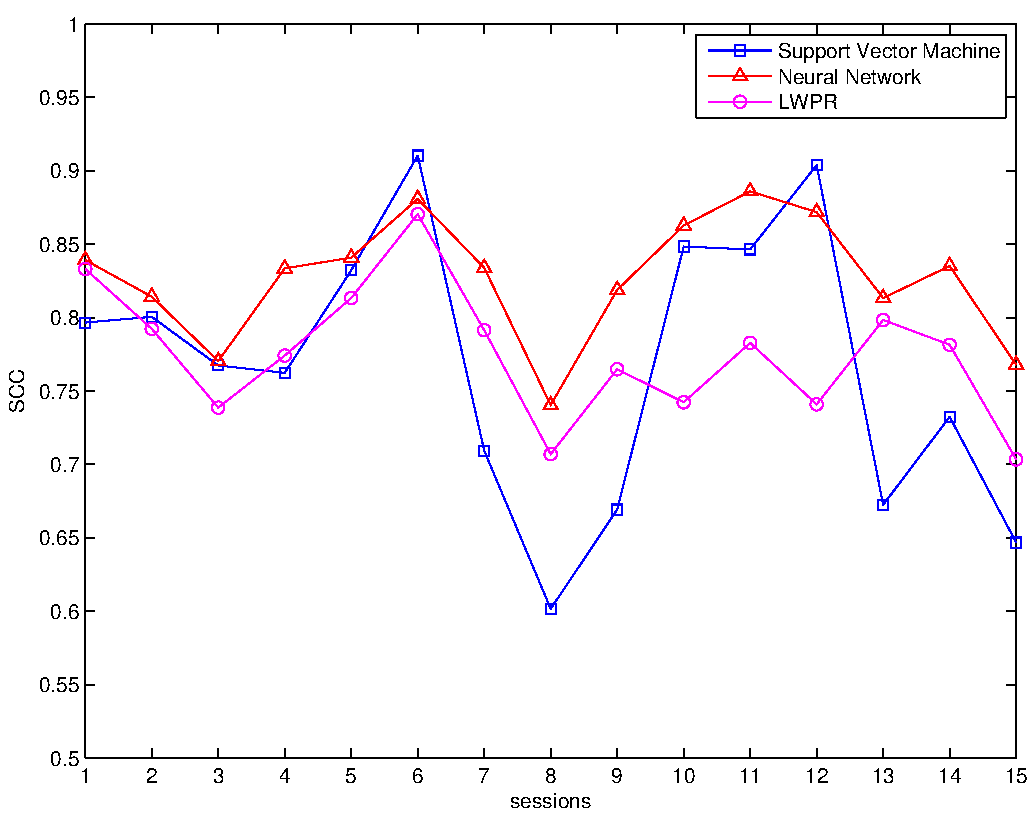
\includegraphics[width=0.45\textwidth]{figs/fig_SCC_regr_resCrossBestOnDay1} &
    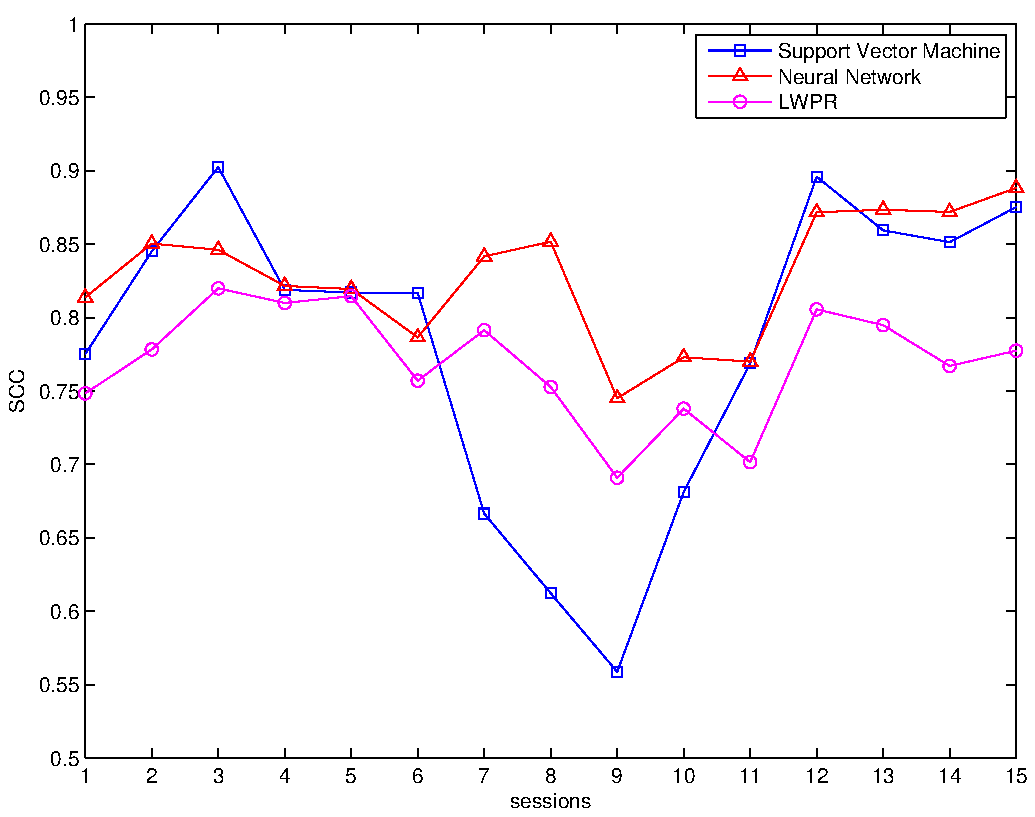
\includegraphics[width=0.45\textwidth]{figs/fig_SCC_regr_resCrossBestOnDay2} \\
     SVM: $0.77 \pm 0.09$ &  SVM: $0.78 \pm 0.11$ \\
      NN: $0.83 \pm 0.04$ &   NN: $0.83 \pm 0.04$ \\
    LWPR: $0.78 \pm 0.05$ & LWPR: $0.77 \pm 0.04$ \\
  \end{tabular}
  \caption{Regression accuracy of best models, day $1$ (left panes)
    and day $2$ (right panes). First row: Mean Squared Error; second
    row: Normalised Root MSE; third row, Squared Correlation Coefficient.}
  \label{fig:best_regr}
\end{figure*}

Figure \ref{fig:best_regr} shows the results; left panes are for day
$1$ and right panes for day $2$. Consider the first row, plotting the
NRMSE for each session: as it is apparent, as it was for
classification, there is no clear advantage of one approach over
another. NNs perform slightly better as far as the NRMSE is concerned,
which is probably the most interesting measure of performance, when
moving to a real setting. Their error is on average $10.54\% \pm
1.41\%$ and $10.01\% \pm 1.93\%$. But as well, both LWPR and SVM
perform quite well, their average errors ranging from $10.54\%$ to
$11.98\%$.

Consider now the second and third rows of the Figure. First of all it
is there is a clear inverse correlation between the MSE and the SCC,
as it is expected: for both days and for all approaches, a larger MSE
corresponds to a lower SCC. Secondly, it is once again clear that the
generalisation performance strongly depends on which data we have used
to train the machines: consider for instance the MSE attained by SVM
on day $1$ (Figure \ref{fig:best_regr}, second row, left pane, blue
curve): the best model was trained upon data coming from sessions $6$
and $12$, although uniformised, and not surprisingly those are the
sessions for which the MSE is minimum; the same effect is present for
the other approaches.

Lastly, in practical terms: the best average MSE obtained by NNs
($6.27\cdot 10^4 \pm 2.36\cdot 10^4$ and $4.76\cdot 10^4 \pm 1.52\cdot
10^4$) corresponds to, in turn, an average error of $5N$ and
$4.36N$. Figure \ref{fig:regression} shows some samples of the force
values obtained from the OFTS, along with the corresponding values
predicted by the best approach, that is, NNs. As one can see, despite
the non perfect correspondence of the two curves, the NN definitely
follows the real target to a remarkable degree of accuracy, for a wide
range of frequencies of the pressing/releasing action. The Figure
shows data taken from three different sessions, in decreasing order of
performance.

\begin{figure*}[!ht] \centering
  \begin{tabular}{ccc}
    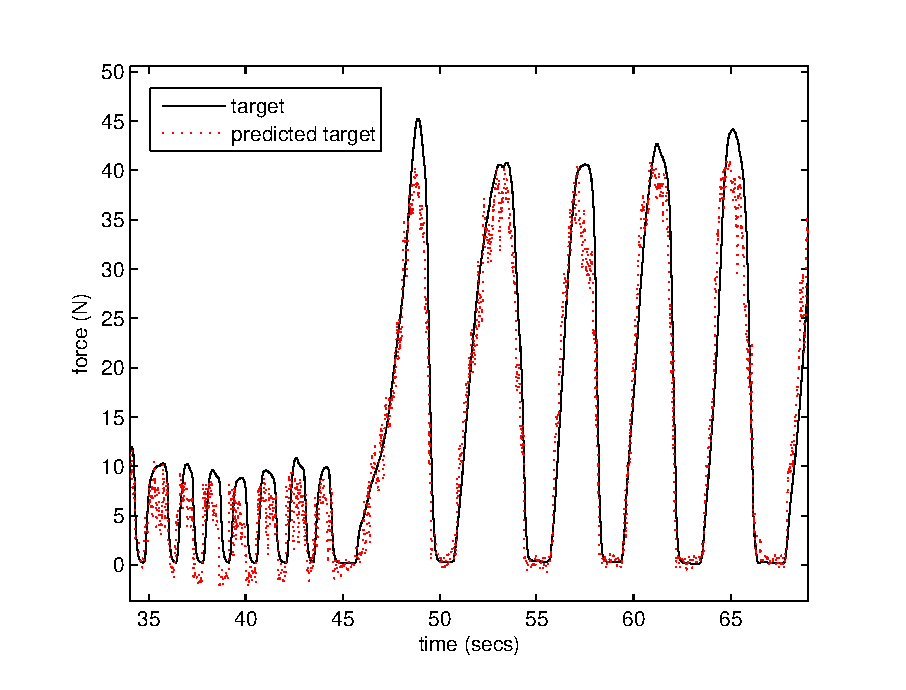
\includegraphics[width=0.30\textwidth]{figs/fig_regression1} &
    \includegraphics[width=0.30\textwidth]{figs/fig_regression2} &
    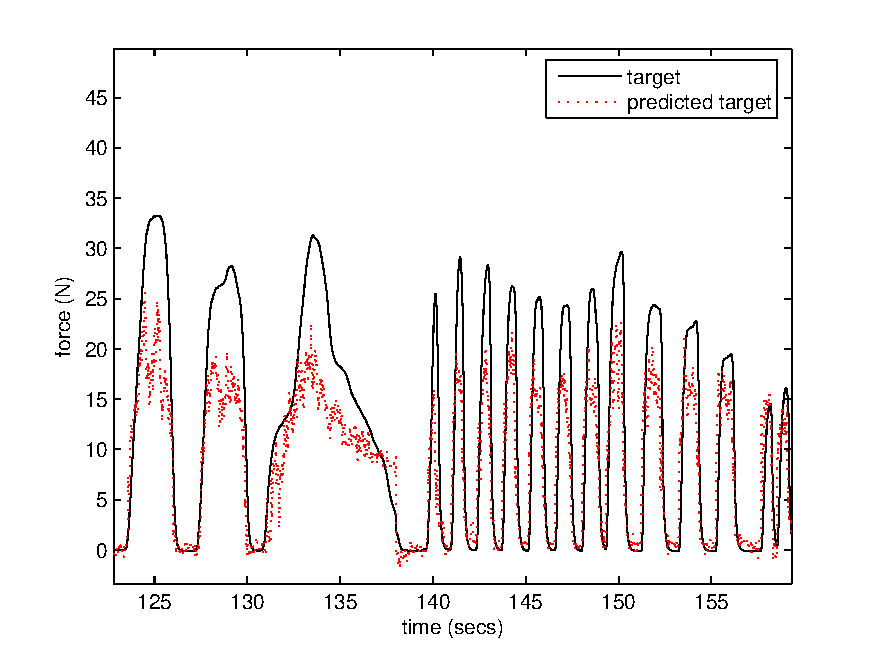
\includegraphics[width=0.30\textwidth]{figs/fig_regression3} \\
    session $6$, day $1$ & session $10$, day $2$ & session $7$, day $1$ \\
    MSE: $4.85\cdot 10^4$ & MSE: $5.48\cdot 10^4$ & MSE: $10.21\cdot 10^4$ \\
  \end{tabular}
  \caption{Examples of the force target value, as guessed by our
    Neural Network.}
  \label{fig:regression}
\end{figure*}

A remarkable point in the Figure is the presence of a ``plateau''
effect, especially in the test with the worst performance, namely
session $7$ of day $1$ (third pane). As is apparent, the predicted
target are mostly wrong in amplitude, being systematically
\emph{lower} than the correct values. Again, this is most likely due
to insufficient sampling in the region of interest.


\subsection{Online Experiments}
\label{subsec:online}
The considerations of the previous Subsection lead to the reasonable
hypothesis that inter-sample distance is the key. Keeping training
sets uniform will result in smaller sets which still contain all
information required for training. Moreover, bad generalisation is
correlated to inter-set distance; therefore uniformisation can be as
well used to retain samples which are far away from the current
training set. We have then implemented an online version of the
uniformisation procedure, in order to test what would happen in a real
setting while the patient is freely moving around.

First of all, we reduced the sampling rate from $256$Hz to about
$25$Hz, since (see Section \ref{subsubsec:electrodes}) the bandwidth
of the EMG signal is limited in our experiment to about $10$Hz. This
got us a total training set of about $153000$ samples. The samples
were naturally chronologically ordered, so that they could be fed to
the system one by one as it would actually happen during continuous
acquisition of data from the patient's activity.

Furthermore, in an online setting no a-priori statistics about the
samples can be assumed. Therefore, as a measure of inter-sample
distance, we dropped the Mahalanobis distance (which requires a good
estimate of the covariance matrix) and resorted to Euclidean distance,
defined in the standard way. Normalisation was still used, as it is
essential for most machine learning methods, but the mean value and
standard deviation of the training sets were evaluated on-the-fly
without keeping the whole sets and re-evaluating them each
time. Testing samples were also normalised according to these
statistics.

We also tested the batch of samples for dimensionality reduction using
PCA, but found that no more than $2$ or $3$ dimensions could be
eliminated. Therefore we dropped the idea, also since PCA would
require, again, an estimate of the covariance matrix of the data set,
which is not available online.

The Online Uniformisation (OU) procedure, then, works like this: we
initially fix a minimum inter-sample distance $d$ and start
with an empty training set $S$. Then each time a new sample $\xx$ is
available, we check whether $dist(\xx,\xx_i)\leq d$, for at
least one $\xx_i \in S$: if this is the case, then $\xx$ is discarded;
otherwise, it is added to $S$.

The first question we were interested in was: does OU give us an
acceptable accuracy \emph{at all times}? That is: does $S$ constitute
a good training set, as the patient explores new regions of the input
space, and more and more samples are seen? In order to answer this
question we considered again the problem of SVM classification, and
let $S$ grow according to the OU procedure. Then, every about $1.5$
minutes of sampled data, that is every $2400$ samples, we trained the
SVM on $S$ and checked its accuracy on a testing set drawn from the
previously seen samples (but not in $S$, of course). This was done $5$
times with different splits of $S$, so to obtain a statistically
meaningful measure of accuracy. We chose to use a mid-range value of
$d = 0.21$ obtained from initial experiments, which would
result in a final training set of about $1800$ samples; moreover, we
used hyperparameters $C = 10^{1.5}$ and $\sigma = 10^{0.5}$, found by
grid search during the preliminary experiments. Figure \ref{fig:inc}
shows the results.

\begin{figure*}[!ht] \centering
  \begin{tabular}{cc}
    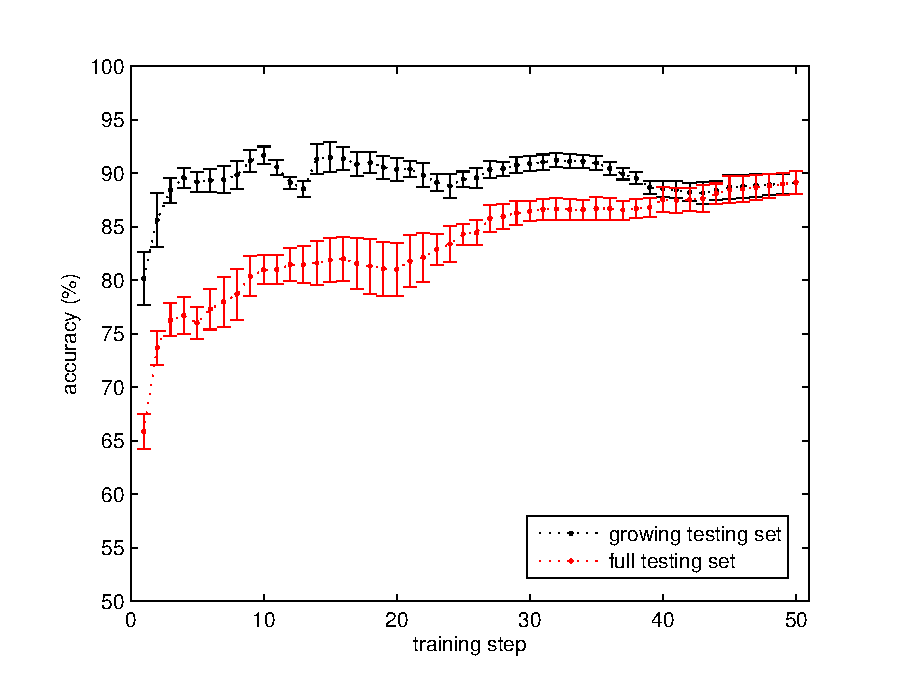
\includegraphics[width=0.45\textwidth]{figs/fig_resInc_OU21} &
    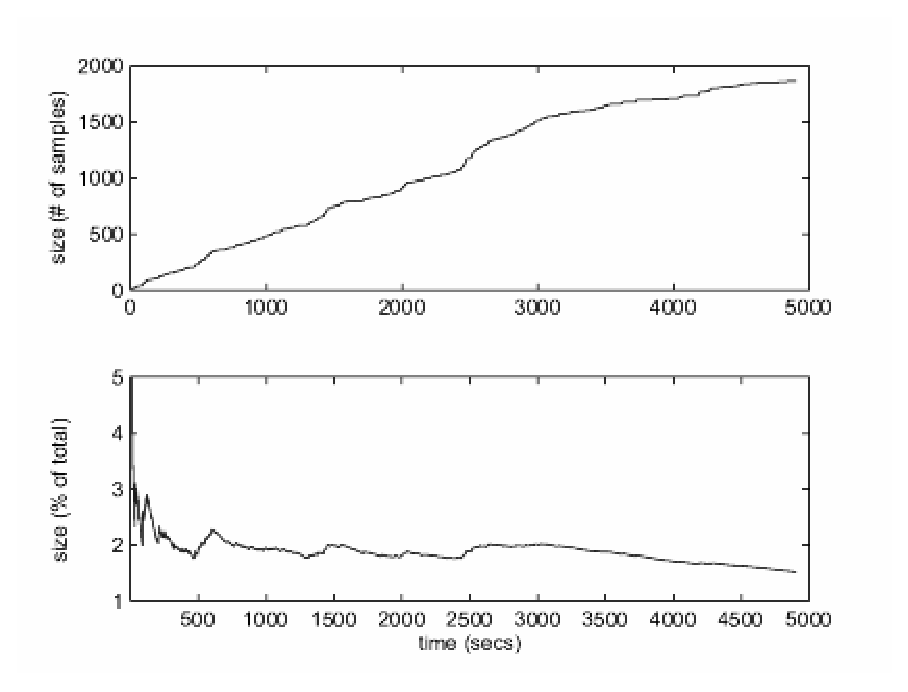
\includegraphics[width=0.45\textwidth]{figs/fig_growth_OU21} \\
    $(a)$ & $(b)$ \\
  \end{tabular}
  \caption{$(a)$: classification accuracy of an SVM, as the training set
    grows according to the OU procedure. \emph{Black curve:}
    growing testing set; \emph{Red curve:} full testing set. $(b)$:
    size of the online uniformised training set: number of samples
    (upper plot), fraction of the whole training set (lower plot).}
  \label{fig:inc}
\end{figure*}

Consider first the black curve in pane $(a)$ of the Figure: it is
apparent that, already after $4$ training steps, that is after some
$6$ minutes, the system can classify with an accuracy of about $90\%$,
as it was the case in the preliminary analysis (accuracy $89.57 \pm
0.94$). Notwithstanding some oscillations, the accuracy remains
substantially constant over the whole test and, at the end, is still
$89.14. \pm 1.05$. Consider now the red curve, representing the
accuracy obtained by the same models but on the \emph{whole} testing
set: now the system is being tested on samples drawn from zones of the
input space it has not yet seen; and, as one would expect, the
accuracy steadily increases, and it finally catches up with that
obtained by testing on the growing testing set.

Consider now pane $(b)$ of the Figure: the upper plot shows the size
of the online uniformised training set as the sample acquisition
proceeds; the lower plot shows the same curve as a fraction of the
full training set size. As time goes on, the OU procedure is letting
the uniform training set grow less and less; the fraction of the full
training set (lower plot) becomes smaller and smaller, being around
$1.5\%$ at the end.

From this we conclude that $(a)$ OU is keeping the training set
remarkably small in absolute terms, and smaller and smaller
percentage-wise, as more and more data is acquired; $(b)$ OU is
``letting in'' only relevant information, since the accuracy is
uniformly high if tested on a growing testing set, and ever growing if
tested upon a full testing set. In other words, the OU procedure is
effective in building a compact and accurate training set for SVM
classification.

What about the other approaches and problems? Figure \ref{fig:allres}
shows an all-inclusive set of results for all problems and approaches
considered, and for various values of the minimum distance threshold,
$d$, which was fixed at $0.21$ in the previous experiment.

\begin{figure*}[!ht] \centering
  \begin{tabular}{cc}
    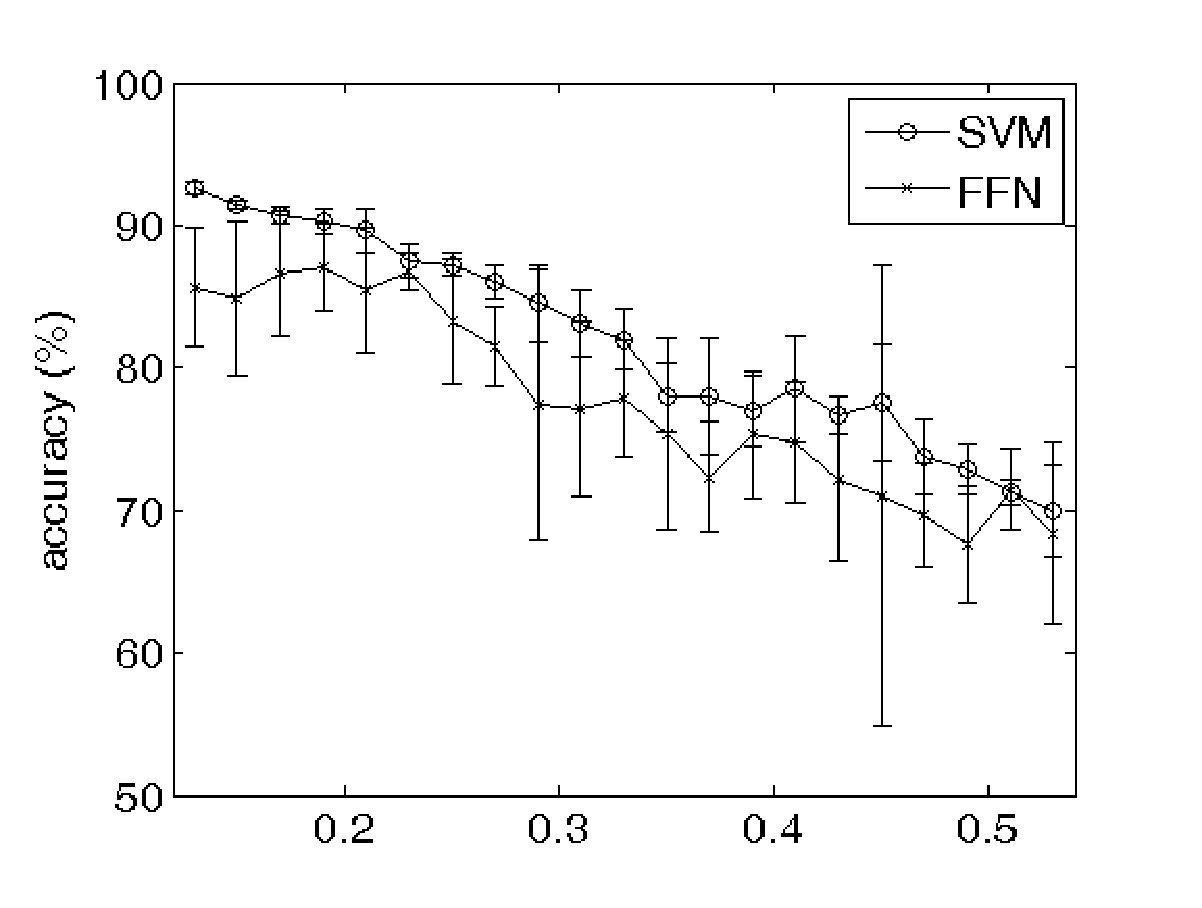
\includegraphics[width=0.45\textwidth]{figs/fig_all1} &
    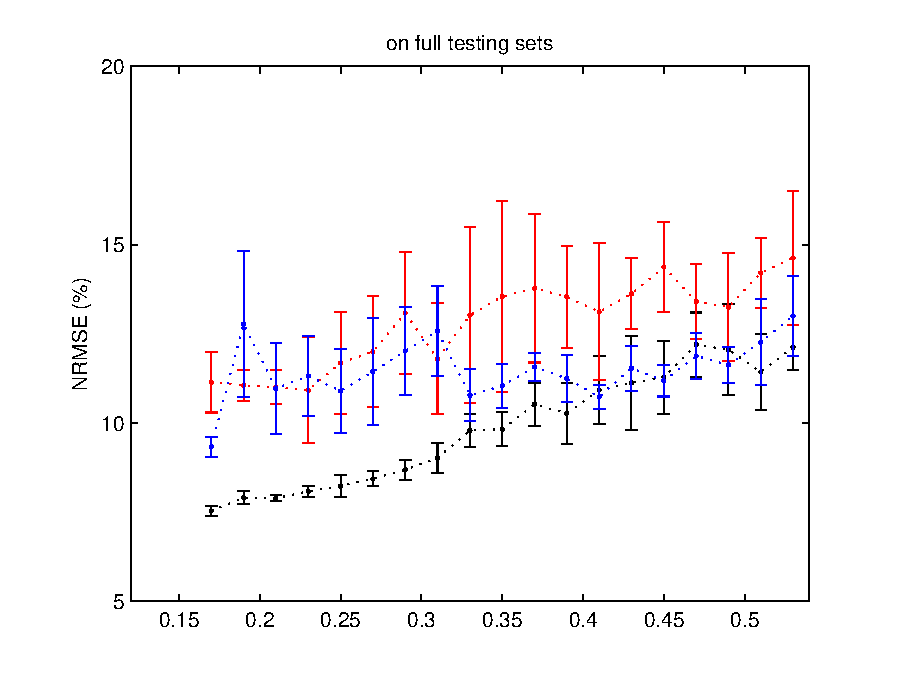
\includegraphics[width=0.45\textwidth]{figs/fig_all2} \\
    $(a)$ & $(b)$ \\
  \end{tabular}
  \caption{Classification and regression results using the OU
  procedure. $(a)$: classification, $(b)$: regression. Compare with
  Figure \ref{fig:TSsize} for the training set sizes.}
  \label{fig:allres}
\end{figure*}

As $d$ is increased from $0.13$ to $0.53$, all approaches show a
decreasing performance, as expected: in classification, the SVM is
uniformly better, going from $92.61\%$ for $d=0.13$ to $70.01\%$ for
$d=0.53$. The standard deviations for the SVM are, also, uniformly
smaller. In regression, again, the SVM is uniformly better than the
other approaches, ranging from $7.09\%$ NRMSE to $12.12\%$, and it
also shows uniformly smaller standard deviations. In both problems,
however, it must be remarked that the error bars largely overlap, at
least for $d>0.4$ for regression. This enables us to conclude that the
SVM is the winning approach overall, but that there are cases in which
another approach can be better.

One last consideration: as $d$ is increased, the size of the training
sets decreases like $d^{-10}$, since we are building a finite
partitioning of a subset of $\RR^{10}$ (see also Figure
\ref{fig:TSsize}, in which the training set size is plotted as a
function of $d$); whereas, it seems that the accuracy of all
approaches, and in both problems, only decreases linearly. This is a
remarkable feature of the OU procedure, since it will always be
possible to choose a $10$-degree polynomially smaller training set and
obtain a machine which is only linearly worse.

\begin{figure}[!ht] \centering
  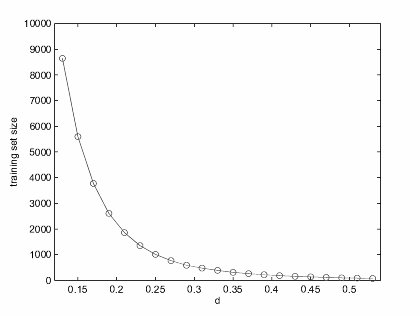
\includegraphics[width=0.45\textwidth]{figs/fig_allSize} \\
  \caption{Online uniformised training set size as $d$ changes.}
  \label{fig:TSsize}
\end{figure}

As a matter of fact, consider once again Figure \ref{fig:allres}, pane
$(b)$: at the far right end we have a SVM which has a still acceptable
error of $12.12\% \pm 0.64\%$, but whose training set, averaged over
the $5$ splits, consists of $77.4$ samples out of the original
$153000$!

Lastly, we compared the results obtained by models trained on uniform
training sets with a simple random selection strategy. In this case,
rather than employing the OU procedure to reduce the training sets,
for each value of $d$ we chose at random the same number of samples
obtained by the OU procedure, and then trained on the models so
obtained. It was expected that, on full training sets, the random
strategy would outperform OU; this is due to the fact that a random
strategy will result in training sets which have the same probability
distribution as the full testing sets; whereas, the OU procedure
produces training sets with a uniform probability distribution. The OU
procedure, on the other hand, is expected to perform better on
\emph{uniform testing sets}, for the same reason. Figure
\ref{fig:rnVSuni} shows the comparative results for SVM classification
and regression, confirming our expectations.

\begin{figure*}[!ht] \centering
  \begin{tabular}{cc}
    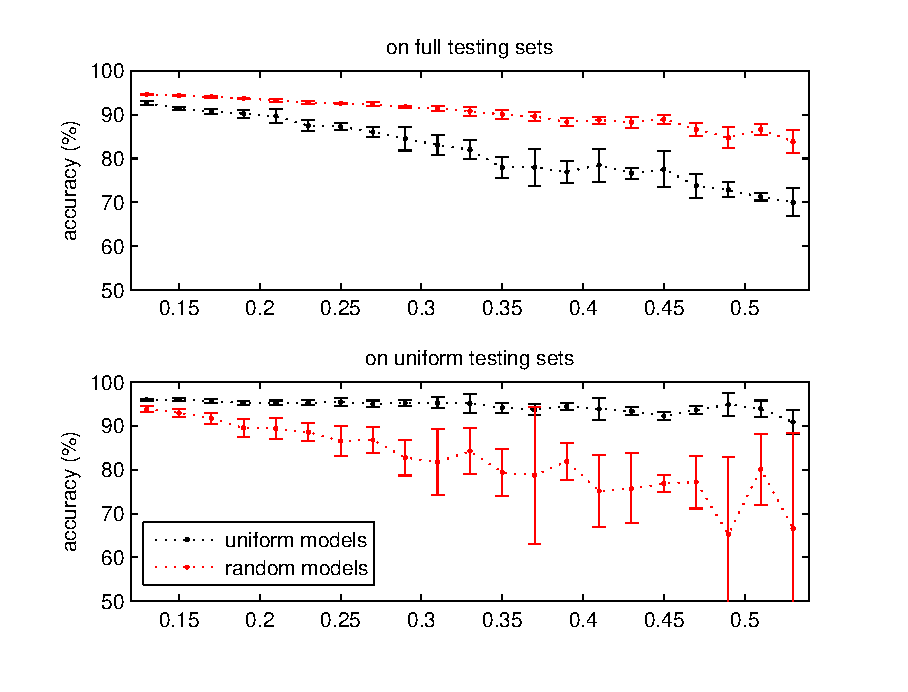
\includegraphics[width=0.45\textwidth]{figs/fig_rnVSuni1} &
    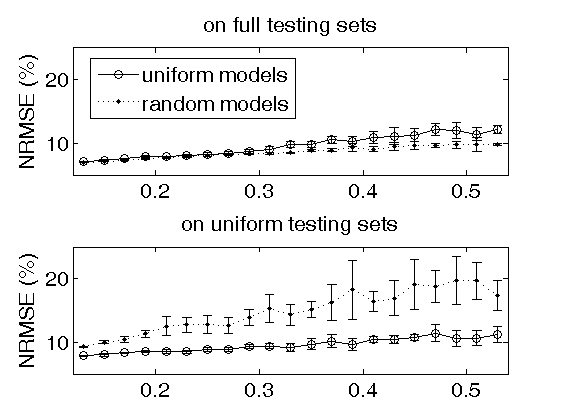
\includegraphics[width=0.45\textwidth]{figs/fig_rnVSuni2} \\
    $(a)$ & $(b)$ \\
  \end{tabular}
  \caption{Classification and regression results, comparing the OU
  procedure with a random sample selection strategy. $(a)$:
    classification, $(b)$: regression.}
  \label{fig:rnVSuni}
\end{figure*}

As one can see, both in classification and in regression, an SVM
trained on uniform training sets will perform uniformly better than
one trained on random training sets, when tested on uniform testing
sets; and uniformly worse when tested on the full training sets. But
the gap is larger in favour of the uniform training sets. This lets us
conclude that uniform training sets will produce models able to
perform well in all situations the patient should move. This is very
useful in a practical setting: for example, picture the situation of a
seldom performed movement, such as turning a door handle; if we were
employing random training sets, we would have a much worse performance
on such a movement. Uniform training sets would make the patient's
life easier.


\subsection{Application to a robotic 4-finger hand}
\label{subsec:application}
The method described above has been used for the control of the DLR
four-finger hand II \cite{ButFisGre2004}. This is a four-finger hand
with thirteen active degrees of freedom: three per finger, and one for
opposition of the thumb.  In the four identical fingers, the motion of
the third phalanx is coupled to that of the second. The actuation
system consists of brushless DC motors, tooth belts, harmonic drive
gears and differential bevel gears in the base joint. The differential
joint allows the use of full power of the two actuators for flexion or
extension, thus allowing the use of optimally small motors, obtaining
30N force at the finger tip. The high joint speed of over
360$^\circ$/s allows for high finger speed, important for, e.g., ball
catching. Besides force and position sensors, we use joint torque
sensors and specially designed potentiometers in each joint.
Furthermore, a tiny six-dimensional force/torque sensor is used in the
finger tip.

\begin{figure}
  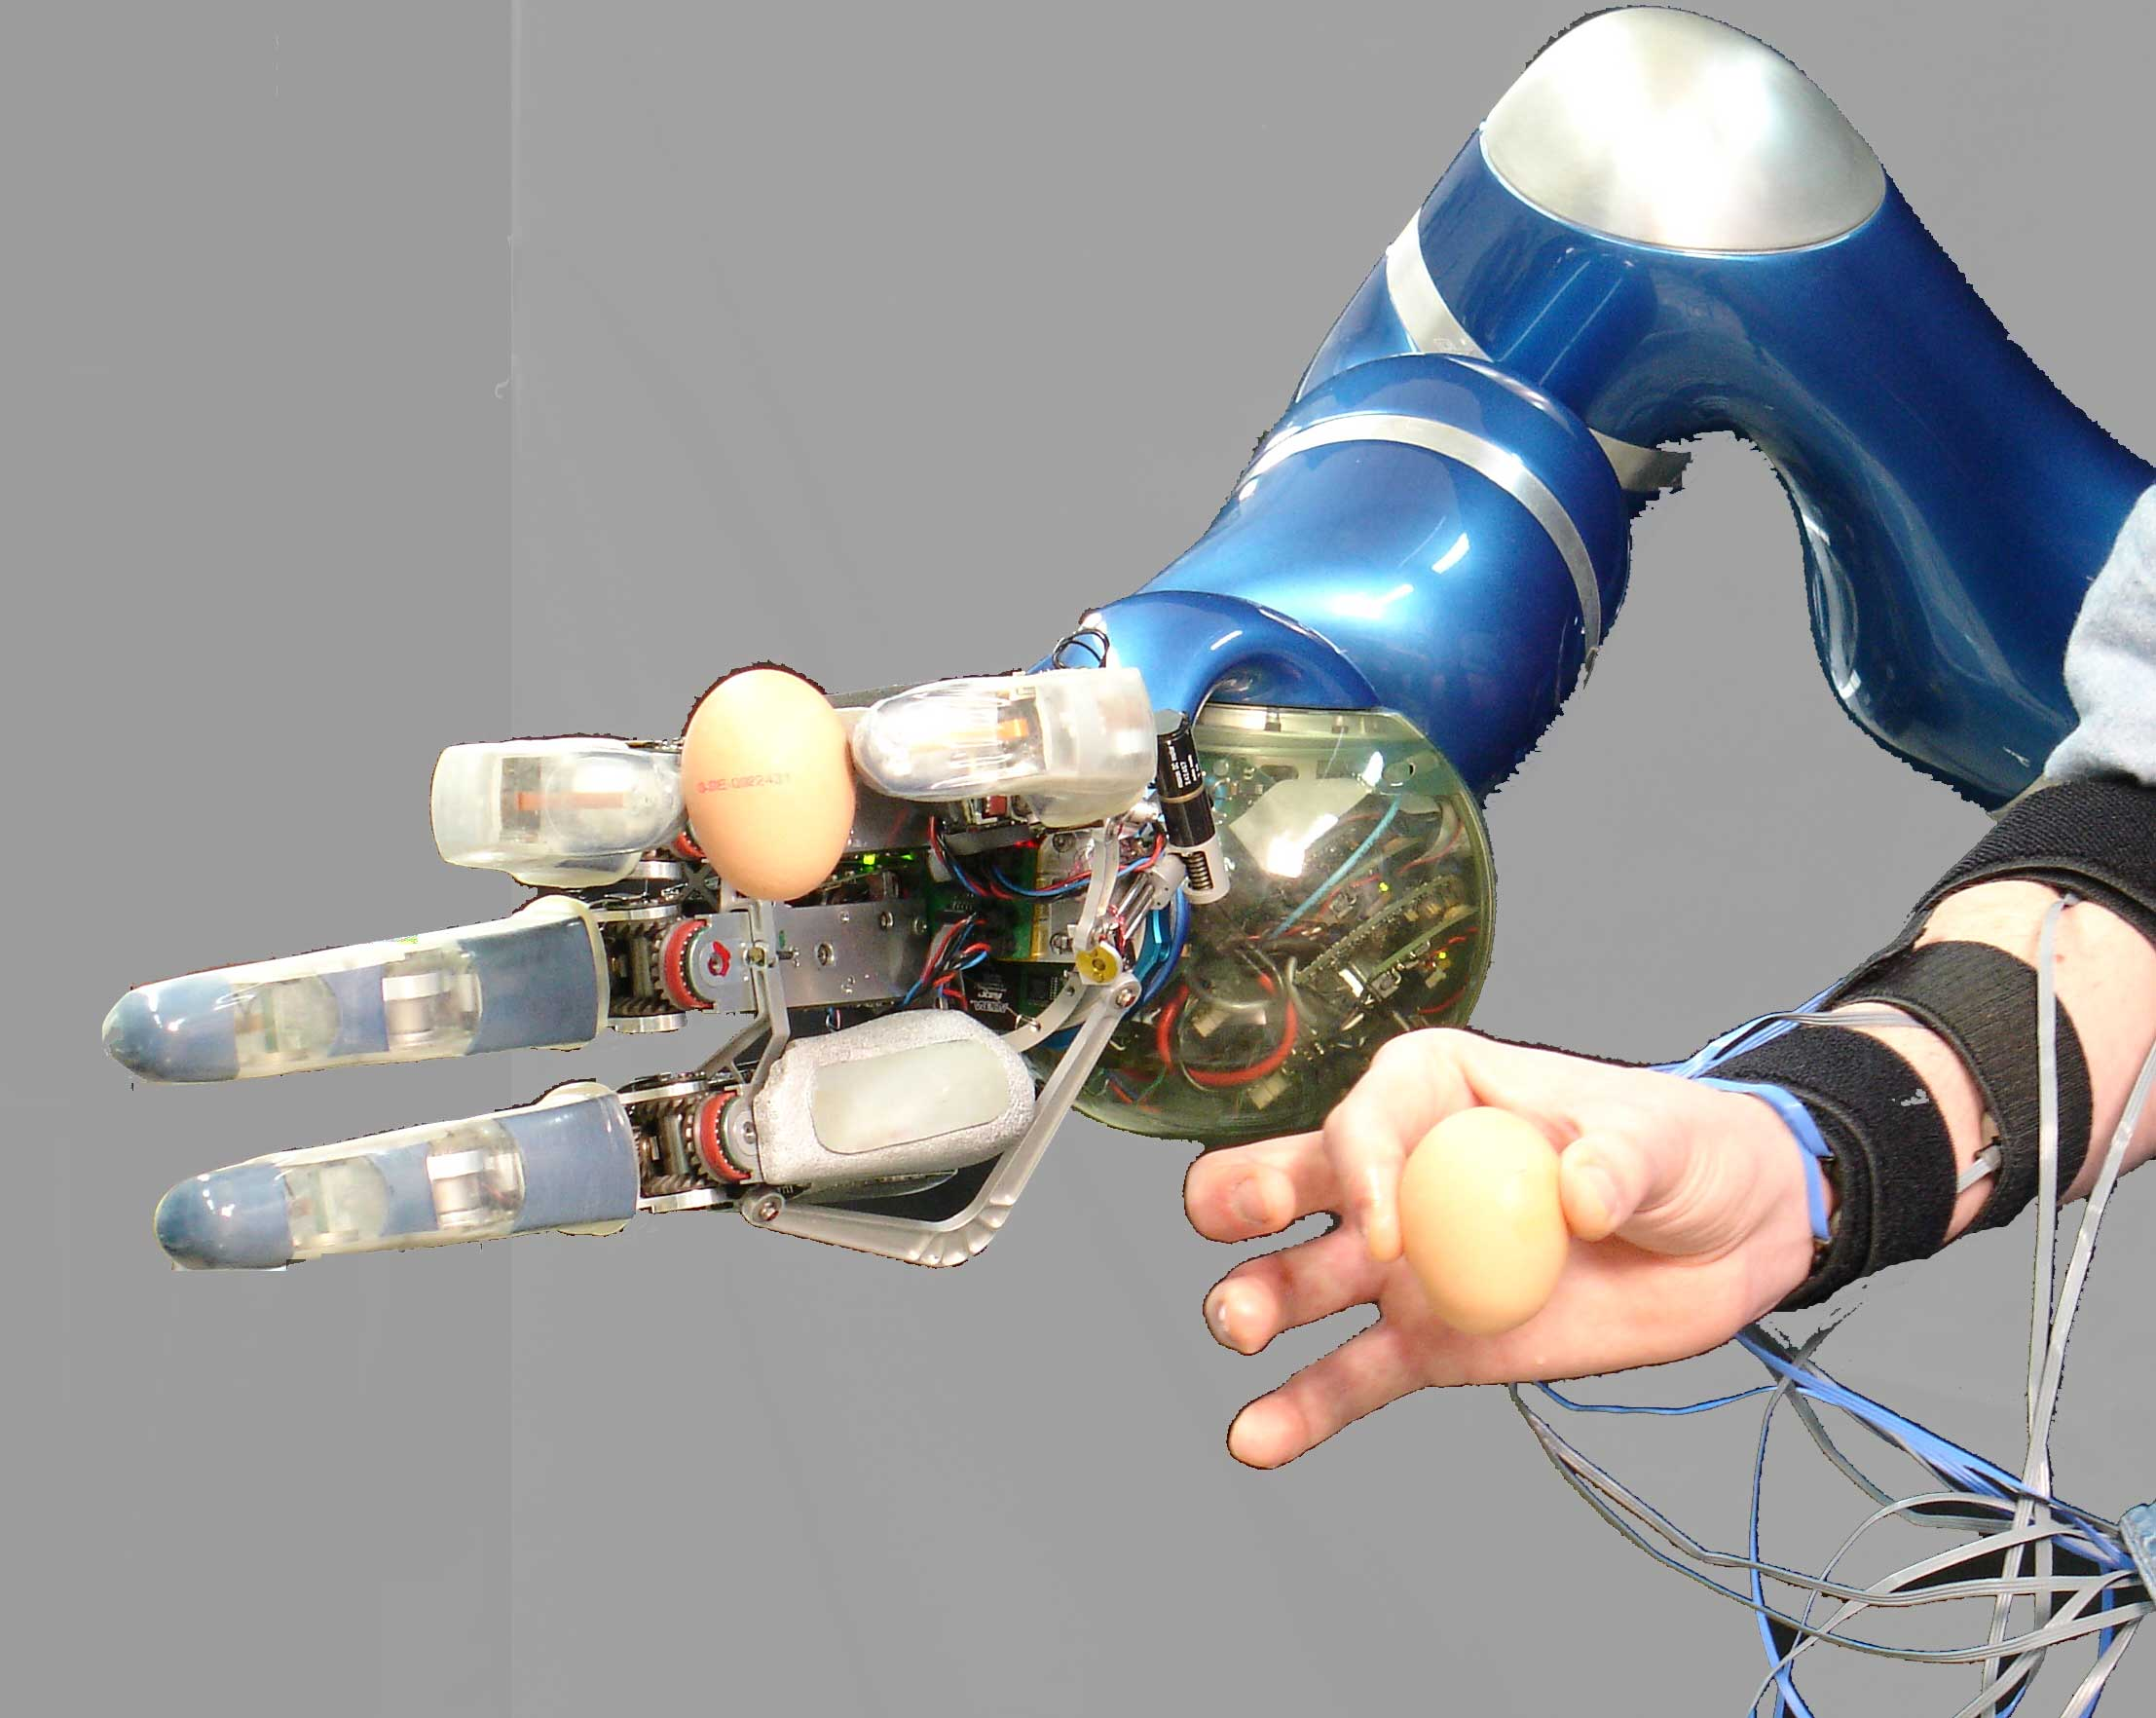
\includegraphics[width=\columnwidth]{figs/egg-in-hand.eps}
  \caption{The DLR four-finger hand II controlled with EMG interface, exerting the right force to hold an egg.}
  \label{fig:egg-hand}
\end{figure}

In the EMG experiment, we used impedance control to exert a force as
generated by the EMG system to hold and grasp object. Example use of
the interface is demonstrated in figure~\ref{fig:egg-hand}. During the
experiment, we verified that the correlation coefficient between the
force applied by the subject and the robot was never less than $80\%$
over a time window of 10 seconds, which let us say that the force
applied by the robot was almost proportional to that applied by the
human subject.


\section{Discussion and Conclusions}
\label{sec:discussion}
Our experimental results, performed on a large data set of about
$153000$ samples, clearly show that the Online Uniformisation
procedure can be used uniformly to obtain dramatically smaller
training sets with no \emph{qualitative} loss of information; in other
words, as more of the input space is sampled, OU keeps the training
set up-to-date and small. OU sets will result in fast and accurate
models of the sought-for EMG-to-hand map. Remarkably, OU works fine
for both grasp classification and force regression, and with all three
different machine learning approaches. Moreover, OU is extremely
simple, being nothing more than an online check of Euclidean distance
in the input space. This check is done so far by considering the new
sample's distance from all samples in the current training set, and
therefore could become unfeasibly heavy as the set grows; but the same
check can be done in constant time using an algorithmic optimisation,
such a hash table.

We believe this is the first step toward the real application of
machine learning to an EMG-driven adaptive, dexterous hand
prosthesis. Let us consider the problems outlined in Subsection
\ref{subsubsec:electrodes}: in this paper we have solved problems
$3$ and $4$. Now, since OU lets us obtain good accuracy with extremely
small training sets, it is not too far-fetched to say that the
solution of problem $2$ is at hand --- in principle, the changing arm
posture can be taken into account simply by sampling more of the input
space. Problem $1$ is, really, of lesser interest, since one patient
only is supposed to ever wear a prosthesis.

As far as force regression is concerned, the results presented above
are, to the best of our knowledge, totally novel. Surprinsingly,
regression from the forearm surcafe EMG signal to the force applied by
the hand had never been attempted before. Given the good performance
obtained by our models, we claim that the relationship between the EMG
signal and the force has been captured by the models, under variable
conditions of muscle fatigue (within one session) and electrode
displacement (within sessions belonging to different groups).

All in all, in this paper we have presented a machine learning
approach to joint classification of grasping and regression on the
applied force, using forearm surface electromyography. The approach is
totally non-invasive, easy to set up and use and it can be applied
from scratch with no previous knowledge of the problem. The Online
Uniformisation procedure can be used to incrementally build a training
set which will result in small and accurate models of the problem.

Our experiments, carried out using a Support Vector Machine with
Gaussian kernel, a Neural Network with sigmoidal activation function
and Locally Weighted Projection Regression, indicate that the approach
achieves, using a training set of about $1800$ samples on a total of
$153000$ (for $d=021$), an average accuracy of around $90\%$ in
classification of grasp types and a normalised root MSE of $7.89\%$ in
prediciton of the force applied during the grasp. Of the tested
approaches, SVM is marginally better than the others, especially when
larger training sets are used. The OU procedure is able to find as
small a training set as $77.4$ samples on average (out of $153000$),
which will still result in a SVM having an NRMSE of $12.12\%$.

Future work can be divided in three steps: firstly, problem $2$ of 
\ref{subsubsec:electrodes} must be taken into account by gathering
more samples, possibly with a more sophisticated EMG/force sensing
setup. Secondly, once a stable model has been built, the actual
position/force control of a mechanical hand must be realised. And
thirdly, in the medium-to-long term, we plan to implant the hand on a
disabled person with extensive experiments to test the real usability
of the proposed approach.


\begin{acknowledgements}
  We thank Giorgio Metta and Giulio Sandini of the
  Italian Institute of Technology for their support.
\end{acknowledgements}

{\small
\bibliographystyle{spbasic}
\bibliography{paper}
}

\end{document}
